\subsection{The Jacobian criterion}

Let \(k\) be a ring, A a \(k\)-algebra, J an ideal of A, and \(\bar{d}:\mathrm{J / J^{2}}\to A /\mathrm{J}\otimes_{\mathrm{A}}\Omega_{k}(\mathrm{A})\) the canonical map. For each A/J-algebra R, we denote

\[
\bar {d} _ {\mathrm{R}}: \mathrm{R} \otimes_ {A / \mathrm{J}} \mathrm{J} / \mathrm{J} ^ {2} \longrightarrow \mathrm{R} \otimes_ {\mathrm{A}} \Omega_ {k} (\mathrm{A})
\]

the R-linear map deduced from \(\bar{d}\). If the k-algebra A/J is formally smooth, \(\bar{d}\) possesses an A-linear retraction (no. 2, remark 1) and \(\bar{d}_{R}\) has an R-linear retraction for every R.

More generally:

Lemma 3.--- Let K be an ideal of A containing J. Suppose there exists an integer m such that \(J \cap K^{m}\) is contained in JK (this condition is satisfied if A is Noetherian). If A/J is formally smooth over k for the K/J-adic topology, the map \(\bar{d}_{A/K}: A/K \otimes_{A/J} J/J^{2} \longrightarrow A/K \otimes_{A} \Omega_{k}(A)\) has an A-linear retraction.

Let C denote the \(k\) -algebra \(\mathrm{A} / (\mathrm{JK} + \mathrm{K}^m)\) ; the ideal \(\mathrm{N} = (\mathrm{J} + \mathrm{K}^m) / (\mathrm{JK} + \mathrm{K}^m)\) of C is square-zero, and the quotient ring C/N identifies with \(\mathrm{A} / (\mathrm{J} + \mathrm{K}^m)\) . Endow C and C/N with the discrete topology, and A/J with the K/J-adic topology. The canonical homomorphism \(\mathrm{A} / \mathrm{J} \to \mathrm{A} / (\mathrm{J} + \mathrm{K}^m)\) is continuous; it therefore has a lifting \(\varphi : \mathrm{A} / \mathrm{J} \to \mathrm{A} / (\mathrm{JK} + \mathrm{K}^m)\) .

The map \(a \mapsto a1_{\mathrm{C}} - \varphi(a1_{\mathrm{A/J}})\) from A to N is then a \(k\)-derivation ( \(n^{\circ} 1\) (prop. 1), hence can be written \(a \mapsto u(da)\) with \(u \in \mathrm{Hom}_{\mathrm{A}}(\Omega_k(\mathrm{A}), \mathrm{N})\). But the hypothesis \(\mathrm{J} \cap \mathrm{K}^m \subset \mathrm{JK}\) implies \(\mathrm{J} \cap (\mathrm{JK} + \mathrm{K}^m) = \mathrm{JK}\), so that the canonical map \(\psi: \mathrm{J/JK} \to \mathrm{N}\) is bijective; there therefore exists \(v \in \mathrm{Hom}_{\mathrm{A/K}}(\mathrm{A/K} \otimes_{\mathrm{A}} \Omega_k(\mathrm{A}), \mathrm{J/JK})\) such that, for a in A, we have \(a1_{\mathrm{C}} = \varphi(a1_{\mathrm{A/J}}) + \psi(v(1 \otimes da))\). Taking a in J, we see that \(v(1 \otimes da)\) is equal to the class of a in J/JK. Since \(\mathrm{A/K} \otimes_{\mathrm{A/J}} \mathrm{J/J}^2\) identifies with J/JK, v is the desired retraction.

The fact that the condition on K is satisfied when the algebra A is Noetherian follows from III, § 3, no. 1, cor. 2 of prop. 1.

Lemma 4.--- Suppose that A is formally smooth over k for the J-adic topology. For A/J to be formally smooth over k, it is necessary and sufficient that the canonical map \(\bar{d}\) has an A-linear retraction.

We already know that if A/J is formally smooth over k, the map \(\bar{d}\) admits an A-linear retraction (no. 2, remark 1). Conversely, suppose that \(\bar{d}\) possesses an A-linear retraction. Let \(\pi: A/J^{2} \to A/J\) be the canonical surjection; by prop. 2 of no. 1, there exists a ring homomorphism \(h: A/J \to A/J^{2}\) such that \(\pi \circ h = 1_{A/J}\). Let C be a k-algebra, N an ideal of C with square zero, and \(\rho: C \to C/N\) the canonical surjection; endow C and C/N with the discrete topology. Let \(u: A/J \to C/N\) be a continuous homomorphism of k-algebras. Since A is formally smooth over k for the J-adic topology, there exists a homomorphism of k-algebras \(v: A \to C\) making the diagram commutative

\pandocbounded{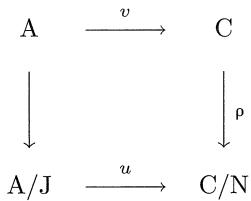
\includegraphics[keepaspectratio]{images/part001_bcdd9d30.jpg}}

where the vertical arrows represent the canonical surjections. We have \(v(\mathrm{J})\subset\mathrm{N}\), hence \(v(\mathrm{J}^{2})\subset\mathrm{N}^{2}=\{0\}\), and v defines, by passing to quotients, a homomorphism \(\bar{v}:\mathrm{A}/\mathrm{J}^{2}\to\mathrm{C}\) which satisfies \(\rho\circ\bar{v}=u\circ\pi\). Then \(\bar{v}\circ h\) is a lifting of u to C.

THEOREM 3.--- Let \(k\) be a ring, A a formally smooth \(k\)-algebra, and J a finitely generated ideal of A; set B=A/J.

\begin{enumerate}
\def\labelenumi{\alph{enumi})}
\tightlist
\item
  Let \(\mathfrak{p}\) be a prime ideal of B and let \(\mathfrak{q}\) be the (prime) ideal of A such that \(\mathfrak{p}=\mathfrak{q}/J\). The following conditions are equivalent:
\end{enumerate}

\begin{enumerate}
\def\labelenumi{(\roman{enumi})}
\item
  the k-algebra \(B_{\mathfrak{p}}\) is formally smooth;
\item
  there exists \(f\in B-\mathfrak{p}\) such that the k-algebra \(B_{f}\) is formally smooth;
\item
  the \(\kappa (\mathfrak{p})\)-linear map
\end{enumerate}

\[
\bar {d} _ {\kappa (\mathfrak {p})}: \kappa (\mathfrak {p}) \otimes_ {\mathrm{B}} \mathrm{J} / \mathrm{J} ^ {2} \rightarrow \kappa (\mathfrak {p}) \otimes_ {\mathrm{A}} \Omega_ {k} (\mathrm{A})
\]

is injective;

\begin{enumerate}
\def\labelenumi{(\roman{enumi})}
\setcounter{enumi}{3}
\tightlist
\item
  there exists an integer \(m \geqslant 0\) , elements \(f_{1}, \ldots, f_{m}\) of J, whose images \((f_{1})_{\mathfrak{q}}, \ldots, (f_{m})_{\mathfrak{q}}\) generate the ideal \(J_{\mathfrak{q}}\) , and k-derivations \(D_{1}, \ldots, D_{m}\) of A such that \(\det(\mathrm{D}_{j}(f_{i})) \not\in \mathfrak{q}\) .
\end{enumerate}

\begin{enumerate}
\def\labelenumi{\alph{enumi})}
\setcounter{enumi}{1}
\item
  The set of prime ideals p of B satisfying the equivalent conditions of (a) is open in Spec(B). For B to be formally smooth over k, it is necessary and sufficient that every prime (respectively maximal) ideal of B satisfy these conditions.
\item
  Suppose A is Noetherian. The conditions of (a) are also equivalent to:
\end{enumerate}

\begin{enumerate}
\def\labelenumi{(\alph{enumi})}
\setcounter{enumi}{21}
\tightlist
\item
  the k-algebra \(B_{\mathfrak{p}}\) is formally smooth for the topology \(\mathfrak{p}B_{\mathfrak{p}}\)-adic.
\end{enumerate}

Moreover, under the conditions of (iv), the ideal \(J_{\mathfrak{q}}\) is completely secant and the sequence \(((f_{1})_{\mathfrak{q}},\ldots,(f_{m})_{\mathfrak{q}})\) is completely secant for \(A_{\mathfrak{q}}\).

Set \(M = J/J^{2}\) and \(N = B \otimes_{A} \Omega_{k}(A)\) . The B-module \(M\) is of finite type, and the B-module \(N\) is projective ( \(n^{\circ} 5\) , cor. 3 of th. 2). For every multiplicative subset \(S\) of \(A\) , the \(k\) -algebra \(S^{-1}A\) is formally smooth ( \(n^{\circ} 2\) , prop. 4, a)). By lemma 4, conditions (i) and (ii) are therefore equivalent respectively to

(i') the map \(\bar{d}_{B_{\mathfrak{p}}}:M_{\mathfrak{p}}\longrightarrow N_{\mathfrak{p}}\) has a \(B_{\mathfrak{p}}\)-linear retraction;

(ii') there exists \(f \in \mathrm{B} - \mathfrak{p}\) such that the map \(\tilde{d}_{\mathrm{B}_f}: \mathrm{M}_f \to \mathrm{N}_f\) has a \(\mathrm{B}_f\)-linear retraction.

Prop. 9 of no. 8 applied to the ring B and to the homomorphism \(\bar{d}:M\to N\) implies the equivalence of conditions (i'), (ii'') and (iii), and also entails the assertions of (b) (using Lemma 4 again). Moreover, (iii) is equivalent to:

(iii') the map \(\kappa(\mathfrak{q})\otimes_{\mathrm{A}}\mathrm{J}\longrightarrow\kappa(\mathfrak{q})\otimes_{\mathrm{A}}\Omega_{k}(\mathrm{A})\) deduced from \(d:\mathrm{J}\to\Omega_{k}(\mathrm{A})\) is injective,

while (iv) can be written as:

(iv') there exists an integer \(m\geqslant 0\), elements \(f_{1},\ldots,f_{m}\) of J whose images generate the ideal \(J_{\mathfrak{q}}\) of \(A_{\mathfrak{q}}\), and elements \(y_{1},\ldots,y_{m}\) of \(\operatorname{Hom}_{\mathrm{A}}(\Omega_{k}(A),A)\) such that \(\det(\langle y_{j},df_{i}\rangle)\notin\mathfrak{q}\).

Since the \(\mathrm{A}\)-module \(\Omega_{k}(A)\) is projective (no. 5, cor. 3 of th. 2), prop. 9 of no. 8, applied to the ring A and to the homomorphism \(d:\mathrm{J}\to\Omega_{k}(A)\) provides the equivalence of (iii') and (iv').

Finally, suppose the ring A is Noetherian. It is clear that (i) implies (v). Under hypothesis (v), Lemma 3 implies that the map

\[
\bar {d} _ {\kappa (\mathfrak {q})}: \kappa (\mathfrak {q}) \otimes_ {\mathrm{B} _ {\mathfrak {p}}} \mathrm{J} _ {\mathfrak {q}} / \mathrm{J} _ {\mathfrak {q}} ^ {2} \longrightarrow \kappa (\mathfrak {q}) \otimes_ {\mathrm{A} _ {\mathfrak {q}}} \Omega_ {k} (\mathrm{A} _ {\mathfrak {q}})
\]

is injective, whence (iii).

Under the conditions of (iv), we have \(m=[\kappa(\mathfrak{q})\otimes_{\mathrm{A}}\mathrm{J}:\kappa(\mathfrak{q})]\) (no. 9, prop. 8). According to th. 2 of no. 5, the ideal \(J_{\mathfrak{q}}\) is completely secant, and the sequence \(((f_1)_{\mathfrak{q}},\ldots,(f_m)_{\mathfrak{q}})\) is completely secant for \(A_{\mathfrak{q}}\) (§ 1, no. 3, cor. 2 of th. 1). This proves c).

COROLLARY 1.--- Let \(k_{0}\) be a ring, \(k\) a Noetherian formally smooth \(k_{0}\)-algebra, and B a local \(k\)-algebra essentially of finite type. If the \(k_{0}\)-algebra B is formally smooth for the topology \(\mathfrak{m}_{\mathrm{B}}\)-adic, it is formally smooth.

There exists an integer \(n\geqslant 0\), a multiplicative subset S of \(k[\mathrm{T}_{1},\ldots,\mathrm{T}_{n}]\), and a surjective \(k\)-homomorphism \(\mathrm{S}^{-1}k[\mathrm{T}_{1},\ldots,\mathrm{T}_{n}]\to\mathrm{B}\). The algebra \(\mathrm{S}^{-1}k[\mathrm{T}_{1},\ldots,\mathrm{T}_{n}]\) is Noetherian and formally smooth over k (no. 3, Example 2 and no. 2, prop. 4, a)), hence over \(k_{0}\) (no. 2, prop. 3, a)). The corollary then follows from Theorem 3, c).

COROLLARY 2.--- Let \(k_{0}\) be a ring, \(k\) a Noetherian formally smooth \(k_{0}\)-algebra, and B a k-algebra essentially of finite type. The set U of prime ideals p of B such that the \(k_{0}\)-algebra \(B_{\mathfrak{p}}\) is formally smooth (for the discrete topology or the topology \(\mathfrak{p}B_{\mathfrak{p}}\)-adic) is open in Spec(B), and the following conditions are equivalent:

\begin{enumerate}
\def\labelenumi{(\roman{enumi})}
\item
  we have U = Spec(B);
\item
  U contains all the maximal ideals of B;
\item
  the \(k_{0}\)-algebra B is formally smooth.
\end{enumerate}

This follows as before from Theorem 3.

Note 1.--- Corollaries 1 and 2 apply in particular when \(k_{0}\) is a field and we are in one of the following two cases:

\begin{enumerate}
\def\labelenumi{\alph{enumi})}
\item
  B is an algebra essentially of finite type over a separable extension of \(k_{0}\) (th. 1 of no. 3);
\item
  B is a \(k_{0}\)-complete Noetherian local algebra whose residue field \(\kappa_{B}\) is a separable extension of \(k_{0}\) (in this case we take for k an algebra of formal power series over \(\kappa_{B}\) of which B is a quotient (no. 3 and IX, § 3, no. 3)).
\end{enumerate}

In each of these cases, it follows from Cor. 2, taking into account Prop. 8 of No. 7 and Prop. 6, b) of § 6, No. 4, that the \(k_0\)-algebra B is formally smooth if and only if it is absolutely regular.

COROLLARY 3 (Zariski). Let \(k\) be a field, A a \(k\)-local regular algebra, and J an ideal of A distinct from A. We assume that the \(k\)-algebra A is essentially of finite type or complete. For the local ring A/J to be regular, it is necessary and sufficient that there exists an integer \(m \geqslant 0\) , elements \(f_1, \ldots, f_m\) of J generating J and derivations D \(_1, \ldots, D_m\) of A such that det(D \(_j(f_i)\) ) \(\not\in \mathfrak{m}_{\mathrm{A}}\). The elements (f \(_1, \ldots, f_m\) ) then form part of a coordinate system of A and the ideal J is prime.

Let \(k_0\) be the prime subfield of \(k\). The \(k_0\)-algebra A is absolutely regular (§ 6, no. 4, Example 1), hence formally smooth (Remark 1 above). For the same reasons, saying that A/J is regular is equivalent to saying that it is a \(k_0\)-algebra formally smooth. The first assertion therefore follows from Theorem 3, which also implies that the sequence \((f_1,\ldots,f_m)\) is completely secant for A. One then applies Proposition 2 of VIII, § 5, no. 3.

Remark 2.--- Under the hypotheses of Cor. 3, the A-module \(\Omega(A)\) is projective (no. 5, Cor. 3 of Theorem 2), hence free; every derivation of A into \(\kappa_{A}\) therefore lifts to a derivation of A. The condition of the statement can thus be expressed as follows: there exists a generating system \((f_{1},\ldots,f_{m})\) of J and derivations \(D_{1},\ldots,D_{m}\) of A into \(\kappa_{A}\) , such that \(\det(D_{j}(f_{i}))\neq0\).

COROLLARY 4 (Zariski).--- Let k be a field and A a k-algebra essentially of finite type or a complete Noetherian local ring. The set of prime ideals p of A such that the local ring A \(_{p}\) is regular is open in Spec(A).

It suffices to apply Remark 1, taking for \(k_0\) the prime subfield of \(k\).

\subsection{Smooth algebras}

Lemma 5.--- Let \(\rho: A \to B\) be a local homomorphism of Noetherian local rings. Suppose that B is essentially of finite type over A. For the A-algebra B to be formally smooth, it is necessary and sufficient that the A-module B be flat and that the \(\kappa_{A}\)-algebra \(\kappa_{A} \otimes_{A} B\) be absolutely regular.

There exists an integer \(n \geqslant 0\), a prime ideal q of \(A[T_{1}, \ldots, T_{n}]\), and a surjective homomorphism h from \(A[T_{1}, \ldots, T_{n}]_{q}\) to B. Let C denote the local A-algebra \(A[T_{1}, \ldots, T_{n}]_{q}\); it is formally smooth ( \(n^{\circ} 3\), Example 2 and \(n^{\circ} 2\), Prop. 4, a)) and flat over A, and one may identify B with the A-algebra C/J, where \(J = \text{Ker}(h)\).

Set \(\overline{\mathrm{C}} = \kappa_{\mathrm{A}} \otimes_{\mathrm{A}} \mathrm{C}\) and \(\overline{\mathrm{B}} = \kappa_{\mathrm{A}} \otimes_{\mathrm{A}} \mathrm{B}\). Suppose B is formally smooth over A. The \(\kappa_{\mathrm{A}}\)-algebra \(\overline{\mathrm{B}}\) is then formally smooth (no. 2, prop. 4, b)), hence absolutely regular (no. 5, cor. 2 of th. 2). Moreover, since \(\overline{\mathrm{C}} / \overline{\mathrm{JC}}\) is identified with \(\overline{\mathrm{B}}\) and since the \(\kappa_{\mathrm{A}}\)-algebra \(\overline{\mathrm{C}}\) is formally smooth, the ideal \(\overline{\mathrm{JC}}\) of \(\overline{\mathrm{C}}\) is completely secant (no. 5, th. 2). It then follows from § 5, no. 6, prop. 6 that the A-module B is flat.

Suppose conversely that B is flat over A and that the \(\kappa_{\mathrm{A}}\)-algebra \(\overline{\mathbf{B}}\) is absolutely regular. Then the \(\kappa_{\mathrm{A}}\)-local algebra \(\overline{\mathbf{B}}\) is formally smooth (Remark 1 of no. 9 with \(k = k_0 = \kappa_{\mathrm{A}}\)). Set \(\overline{\mathbf{J}} = \kappa_{\mathrm{A}} \otimes_{\mathrm{A}} \mathrm{J}\); since B is a flat A-module, the canonical map \(\overline{\mathbf{J}} \to \overline{\mathbf{J}}\overline{\mathbf{C}}\) is bijective and \(\overline{\mathbf{B}}\) is identified with \(\overline{\mathbf{C}}/\overline{\mathbf{J}}\). It follows (Remark 1 of no. 2) that the canonical map

\[
\overline {{\mathrm{J}}} / \overline {{\mathrm{J}}} ^ {2} \longrightarrow \overline {{\mathrm{B}}} \otimes_ {\overline {{\mathrm{C}}}} \Omega_ {\kappa_ {\mathrm{A}}} (\overline {{\mathrm{C}}})
\]

is injective and admits a retraction. Now \(\overline{\mathrm{J}}/\overline{\mathrm{J}}^{2}\) is identified with \(\kappa_{\mathrm{A}}\otimes_{\mathrm{A}}\mathrm{J}/\mathrm{J}^{2}\), hence with \(\overline{\mathrm{B}}\otimes_{\mathrm{B}}\mathrm{J}/\mathrm{J}^{2}\). On the other hand, the \(\overline{\mathrm{C}}\)-module \(\Omega_{\kappa_{\mathrm{A}}}(\overline{\mathrm{C}})\) is canonically isomorphic to \(\overline{\mathrm{C}}\otimes_{\mathrm{C}}\Omega_{\mathrm{A}}(\mathrm{C})\) (A, III, p. 136, prop. 20), hence \(\overline{\mathrm{B}}\otimes_{\overline{\mathrm{C}}}\Omega_{\kappa_{\mathrm{A}}}(\overline{\mathrm{C}})\) is canonically isomorphic to \(\overline{\mathrm{B}}\otimes_{\mathrm{C}}\Omega_{\mathrm{A}}(\mathrm{C})\). Passing to the quotient by the maximal ideal of \(\overline{\mathrm{B}}\), one obtains an injective homomorphism

\[
\kappa_ {B} \otimes_ {B} J / J ^ {2} \longrightarrow \kappa_ {B} \otimes_ {C} \Omega_ {A} (C)
\]

which is precisely \(\bar{d}_{\kappa_{\mathrm{B}}}\). Thus B is formally smooth over A (th. 3).

THEOREM 4.--- Let A be a Noetherian ring and B an A-algebra essentially of finite type. The following conditions are equivalent:

\begin{enumerate}
\def\labelenumi{(\roman{enumi})}
\item
  the A-algebra B is formally smooth;
\item
  for every \(\mathfrak{q} \in \operatorname{Spec}(\mathrm{B})\) , the A-algebra \(\mathrm{B}_{\mathfrak{q}}\) is formally smooth (resp. formally smooth for the topology \(\mathfrak{q}\mathrm{B}_{\mathfrak{q}}\) -adic);
\item
  the A-module B is flat and, for every \(\mathfrak{p} \in \operatorname{Spec}(A)\) , the \(\kappa(\mathfrak{p})\) -algebra \(\kappa(\mathfrak{p}) \otimes_{A} B\) is absolutely regular;
\item
  the A-module B is flat and, for every regular A-algebra R, the ring R ⊗\_A B is regular;
\item
  the A-module B is flat and the kernel of the homomorphism \(\mu:B\otimes_{A}B\to B\) defined by \(\mu(x\otimes y)=xy\) is a completely secant ideal.
\end{enumerate}

The equivalence of (i) and (ii) follows from cor. 2 of th. 3 (no. 9).

(i)⇒(v): suppose the A-algebra B is formally smooth. Let q be a prime ideal of B, and let p be its inverse image in A. The \(A_{\mathfrak{p}}\)-algebra \(B_{\mathfrak{q}}\) is formally smooth (prop. 4, a) of no. 2), hence flat (Lemma 5); consequently the A-module B is flat (II, § 3, no. 4, prop. 15). On the other hand, the ring B ⊗A B is Noetherian (§ 6, no. 1, cor. of prop. 2), so the ideal Ker μ is completely secant by cor. 3 of th. 2 (no. 5).

(v)⇒(iii): suppose condition (v) is satisfied. Set I = Ker(μ). Let p ∈ Spec(A). The map

\[
1 \otimes \mu : \kappa (\mathfrak {p}) \otimes_ {\mathrm{A}} (\mathrm{B} \otimes_ {\mathrm{A}} \mathrm{B}) \rightarrow \kappa (\mathfrak {p}) \otimes_ {\mathrm{A}} \mathrm{B}
\]

is identified with the map

\[
\mu_ {\mathfrak {p}}: (\kappa (\mathfrak {p}) \otimes_ {\mathrm{A}} \mathrm{B}) \otimes_ {\kappa (\mathfrak {p})} (\kappa (\mathfrak {p}) \otimes_ {\mathrm{A}} \mathrm{B}) \rightarrow \kappa (\mathfrak {p}) \otimes_ {\mathrm{A}} \mathrm{B}
\]

deduced from the multiplication of the \(\kappa(\mathfrak{p})\) -algebra \(\kappa(\mathfrak{p})\otimes_{\mathrm{A}}\mathrm{B}\) . The ideal \(\operatorname{Ker}(\mu_{\mathfrak{p}})\) is identified with \(\mathrm{I}(\kappa(\mathfrak{p})\otimes_{\mathrm{A}}(\mathrm{B}\otimes_{\mathrm{A}}\mathrm{B}))\) . It is completely secant since the A-module B is flat ( \(\S 5\) , no. 6, prop. 6). Assertion (iii) then follows from prop. 8 of \(\S 6\) , no. 5.

(iii)⇒(ii): let q be a prime ideal of B, and p its inverse image in A. Under the hypotheses of (iii), the A \(_{p}\) -module B \(_{q}\) is flat, and the κ(p)-algebra κ(p) ⊗A \(_{p}\) B \(_{q}\) , which is identified with a ring of fractions of κ(p) ⊗A B, is absolutely regular (§ 6, no. 4, prop. 6). It follows from lemma 5 that B \(_{q}\) is formally smooth over A \(_{p}\) , hence over A (no. 2, prop. 3 and 4).

(iii)⇒(iv): let us place ourselves under the hypotheses of (iii). Let R be a regular A-algebra. The R-module R ⊗A B is flat (I, § 2, no. 7, cor. 2 to prop. 8). Let r be a prime ideal of R and p its inverse image in A; the ring κ(r)⊗R(R⊗AB), which is identified with κ(r)⊗κ(p) (κ(p)⊗A B), is regular (§ 6, no. 4, cor. 2 of prop. 7). The ring R ⊗A B is therefore regular (§ 4, no. 5, cor. of prop. 9).

(iv)⇒ (iii): let p be a prime ideal of A and let k be an extension of κ(p); under the hypotheses of (iv), the ring \(k \otimes_{\kappa(\mathfrak{p})} (\kappa(\mathfrak{p}) \otimes_{\mathrm{A}} \mathrm{B})\) , which is identified with \(k \otimes_{A} B\) , is regular, whence (iii).

DEFINITION 2.--- Let A be a Noetherian ring. An A-algebra B is said to be smooth if it is essentially of finite type and if it satisfies the equivalent conditions of Theorem 4.

PROPOSITION 10.--- Let A be a Noetherian ring.

\begin{enumerate}
\def\labelenumi{\alph{enumi})}
\item
  Let A' be a Noetherian A-algebra and B a smooth A-algebra. Then the A'-algebra A' ⊗\_A B is smooth.
\item
  Let B be a smooth A-algebra and C a smooth B-algebra. Then the A-algebra C is smooth.
\item
  Let B and C be two smooth A-algebras. Then the A-algebra B ⊗A C is smooth.
\end{enumerate}

This follows from prop. 4 of no. 2 and the analogous statements for algebras essentially of finite type (§ 6, no. 1).

Examples.--- 1) Smooth algebras over a field \(k\) are precisely the essentially finite-type and absolutely regular \(k\)-algebras.

\begin{enumerate}
\def\labelenumi{\arabic{enumi})}
\setcounter{enumi}{1}
\tightlist
\item
  Let A be a Noetherian ring, \(\mathbf{T} = (\mathrm{T}_i)_{i\in I}\) a finite family of indeterminates. The A-algebra A{[}T{]} is smooth. More generally, let \(\mathrm{F}_1,\ldots ,\mathrm{F}_m\) of elements of A{[}T{]}, and let B be the A-algebra A{[}T{]}/ \((\mathrm{F}_1,\dots ,\mathrm{F}_m)\). If in every maximal ideal \(\mathfrak{n}\) of B the class (mod. \(\mathfrak{n}\) ) of the matrix \(\left(\frac{\partial\mathrm{F}_j}{\partial\mathrm{T}_i}\right)\) is of rank \(m\) , the A-algebra B is smooth (th. 3 of no. 9).
\end{enumerate}

\section{Duality of modules of finite length}

\subsection{Indecomposable injective modules}

Let A be a ring. The relation “I is a class of indecomposable injective A-modules” is collectivizing (A, X, p. 21, cor. 1); we shall denote by \(\mathcal{I}(A)\) the set of classes of indecomposable injective A-modules.

PROPOSITION 1.--- Let A be a Noetherian ring. For every prime ideal p of A, let \(e_{\mathfrak{p}}: \mathrm{A}/\mathfrak{p} \to \mathrm{I}(\mathfrak{p})\) be an injective envelope of \(\mathrm{A}/\mathfrak{p}\) (A, X, § 1, no. 9).

\begin{enumerate}
\def\labelenumi{\alph{enumi})}
\item
  The A-modules I(p) are indecomposable.
\item
  Let I be an indecomposable injective A-module; the set Ass(I) is reduced to a single element.
\item
  The map \(\mathfrak{p} \mapsto \operatorname{cl}(\operatorname{I}(\mathfrak{p}))\) is a bijection of \(\operatorname{Spec}(\operatorname{A})\) onto \(\mathcal{I}(A)\). The inverse bijection associates to an element I of \(\mathcal{I}(\operatorname{A})\) the unique element of \(\operatorname{Ass}(\operatorname{I})\).
\end{enumerate}

Let \(\mathfrak{p} \in \operatorname{Spec}(A)\); let us prove that the module \(I(\mathfrak{p})\) is indecomposable. By A, X, p. 21, cor. 2, it suffices to prove that if \(\mathfrak{a}\) and \(\mathfrak{b}\) are ideals of A containing \(\mathfrak{p}\) and distinct from \(\mathfrak{p}\), the ideal \(\mathfrak{a} \cap \mathfrak{b}\) is distinct from \(\mathfrak{p}\) ; or if \(a\) is an element of \(\mathfrak{a} - \mathfrak{p}\) and \(b\) is an element of \(\mathfrak{b} - \mathfrak{p}\) the product \(ab\) belongs to \((\mathfrak{a} \cap \mathfrak{b}) - \mathfrak{p}\).

Let I be an indecomposable injective A-module, and let p, q be elements of Ass(I). Then I contains a submodule M isomorphic to A/p and a submodule N isomorphic to A/q. We have M ∩ N ≠ 0 (A, X, p. 21, prop. 14); for every nonzero element x of M ∩ N, we have p = Ann x = q. Since Ass(I) is not empty (IV, § 1, n° 1, cor. 1 of prop. 2), it is reduced to a single element p(I).

We have thus defined two maps. \(\mathfrak{p} \mapsto \operatorname{cl}(I(\mathfrak{p}))\) of \(\operatorname{Spec}(A)\) in \(\mathcal{I}(A)\) and \(I \mapsto \mathfrak{p}(I)\) of \(\mathcal{I}(A)\) in \(\operatorname{Spec}(A)\); let us prove that these two maps are inverse bijections of each other. Let \(\mathfrak{p} \in \operatorname{Spec}(A)\) ; then \(\mathfrak{p}\) belongs to \(\operatorname{Ass}(I(\mathfrak{p}))\), and it is therefore the unique element of \(\operatorname{Ass}(I(\mathfrak{p}))\). Let \(I\) be an indecomposable injective A-module, and \(\mathfrak{p}\) the unique element of \(\operatorname{Ass}(I)\) ; then \(I\) is an injective envelope of \(A/\mathfrak{p}\) (A, X, p. 21, prop. 14). This completes the proof of the proposition.

Remark 1.—Let I be an indecomposable injective A-module, and let p be the unique element of Ass(I); by Prop. 1, I contains a submodule isomorphic to A/p of which it is an injective envelope. In general such a submodule is not unique, as one sees by taking A = Z, p = 0, I = Q.

For every prime ideal \(\mathfrak{p}\) of \(\mathrm{A}\), let us choose, as above, an injective envelope \((\mathrm{I}(\mathfrak{p}), e_{\mathfrak{p}})\) of \(\Lambda/\mathfrak{p}\). By \(\mathrm{A}\), X, p. 22, th. 3, we have:

THEOREM 1.--- Let A be a Noetherian ring. For every injective A-module I, there exists one and only one family of cardinals \((a_{\mathfrak{p}})_{\mathfrak{p}\in\operatorname{Spec}(\mathrm{A})}\), such that I is isomorphic to \(\bigoplus_{\mathfrak{p}}\mathrm{I}(\mathfrak{p})^{(a_{\mathfrak{p}})}\).

By IV, § 1, no. 1, cor. 1 of prop. 3, the set Ass(I) is then the support of the family \((a_{\mathfrak{p}})\) .

Remark 2. Let \(A\) be a Noetherian ring, M an A-module, \(e: \mathrm{M} \to \mathrm{I}\) an injective envelope of M. The set Ass(M) is equal to Ass(I): indeed, the inclusion Ass(M) ⊂ Ass(I) is evident. On the other hand, if \(\mathfrak{p}\) is an element of Ass(I), I contains a submodule N isomorphic to \(A/\mathfrak{p}\) ; since the \(A\)-module \(e^{-1}(\mathrm{N})\) is nonzero, we have \(\operatorname{Ass}(e^{-1}(\mathrm{N})) = \{\mathfrak{p}\}\). This proves that \(\mathfrak{p}\) is associated with \(e^{-1}(\mathrm{N})\), hence to M, whence our assertion.

Let us adopt the notation of the theorem, and suppose moreover that Ass(M) is finite. For every \(\mathfrak{q} \in \operatorname{Ass}(M)\) let us denote by \(Q_{\mathfrak{q}}\) the intersection with M of \(\bigoplus_{\mathfrak{p} \in \operatorname{Ass}(M) - \{\mathfrak{q}\}} I(\mathfrak{p})^{(a_{\mathfrak{p}})}\). Then \((Q_{\mathfrak{q}})_{\mathfrak{q} \in \operatorname{Ass}(M)}\) is a reduced primary decomposition of 0 in M (IV, § 2, n° 3, def. 3). Indeed, we have \(\cap Q_{\mathfrak{q}} = 0\); as \(M/Q_{\mathfrak{q}}\) is identified with a nonzero submodule of \(I(\mathfrak{q})^{(a_{\mathfrak{q}})}\), one has \(\operatorname{Ass}(M/Q_{\mathfrak{q}}) = \{\mathfrak{q}\}\) and it suffices to apply prop. 4 of loc. cit.

Example.--- Let A be a principal ideal ring, and let K be its field of fractions. The injective A-modules are the divisible A-modules (A, X, p. 17, cor. 2). The A-module K is an injective envelope of A (A, X, p. 20, example 1). Let \(p\) be an extremal element of A, and \(\mathfrak{p}\) the (maximal) ideal \(Ap\). Let us denote by \(e: A/\mathfrak{p} \longrightarrow K/A_{\mathfrak{p}}\) the homomorphism that maps the class of an element \(a \in A\) to the class of \(a/p\). Let us prove that \((K/A_{\mathfrak{p}}, e)\) is an injective envelope of \(A/\mathfrak{p}\). The homomorphism \(e\) is injective. The A-module \(K/A_{\mathfrak{p}}\) is a quotient of a divisible module, hence is divisible. Let \(x\) be a nonzero element of \(K/A_{\mathfrak{p}}\) ; it is the class of an element \(a/p^n\) of K, with \(a \in A - \{0\}\) and \(n \geqslant 1\) (A, VII, p. 10, th. 2). We then have \(p^{n-1}x = e(a)\) , hence \(e(Ax) \neq 0\), which proves our assertion.

It then follows from th. 1 that every divisible A-module is a direct sum of A-modules isomorphic to K or to \(K/A_{p}\) for a maximal (principal) ideal p of A.

\subsection{Structure of indecomposable injective modules}

Lemma 1.--- Let A be a ring, with a an ideal of A, and I an A-module. For every integer \(n \geqslant 0\) let us denote by \(I_{n}\) the submodule of I consisting of the elements annihilated by \(a^{n}\).

\begin{enumerate}
\def\labelenumi{\alph{enumi})}
\item
  Suppose the A-module I is injective. Then the \(\mathrm{A} / \mathfrak{a}^n\)-module \(\mathrm{I}_n\) is injective for every \(n \geqslant 0\).
\item
  Suppose that the ring A is Noetherian, and that for every \(n \geqslant 0\) the \(\mathrm{A} / \mathfrak{a}^n\) -module \(\mathrm{I}_n\) be injective. Then the union of the \(\mathrm{I}_n\) is an injective A-module.
\item
  The \(\mathbf{A} / \mathfrak{a}^n\) -module \(\mathrm{I}_n\) is isomorphic to \(\operatorname{Hom}_{\mathbf{A}}(\mathbf{A} / \mathfrak{a}^n, \mathbf{I})\), which is injective (A, X, p. 18, prop. 11).
\item
  Let J be the union of the \(I_{n}\), b an ideal of A, and \(f : b \to J\) an A-homomorphism. It remains (A, X, p. 16, prop. 10) of proving that there exists an element x of J such that one has \(f(b) = bx\) for every \(b \in b\). Since b is of finite type, there exists an integer n such that one has \(f(\mathfrak{b}) \subset \mathrm{I}_{n}\) , that is \(f(\mathfrak{a}^{n}\mathfrak{b}) = 0\) . According to cor. 2 of prop. 1 of III, § 3, no. 1, there exists an integer \(m \geqslant n\) such that \(a^{m} \cap b \subset a^{n}b\) , hence \(f(\mathfrak{a}^{m} \cap \mathfrak{b}) = 0\) . Then f induces an A/\(a^{m}\)-linear homomorphism from \(\mathfrak{b}/(\mathfrak{a}^{m} \cap \mathfrak{b})\) into \(I_{m}\); since the A/ \(a^{m}\)-module \(I_{m}\) is injective, there exists an element x of \(I_{m}\) such that one has \(f(b) = bx\) for every \(b \in b\) , whence b).
\end{enumerate}

Let \(\mathfrak{a}\) be an ideal of A; in what follows we shall agree to set \(\mathfrak{a}^n = \mathrm{A}\) for every integer \(n \leqslant 0\). Let E be an A-module. For every \(n \in \mathbf{Z}\) let us denote by \(\mathrm{E}_n\) the submodule of E consisting of the elements annihilated by \(\mathfrak{a}^n\); let \(\mathrm{gr}^{\mathfrak{a}}(\mathrm{E})\) be the graded A-module of type \(\mathbf{Z}\) such that \(\mathrm{gr}^{\mathfrak{a}}(\mathrm{E})_m = \mathrm{E}_{-m+1}/\mathrm{E}_{-m}\) for every integer \(m\). The module \(\mathrm{gr}^{\mathfrak{a}}(\mathrm{E})_m\) is zero for \(m \geqslant 1\) , and \(\mathrm{gr}^{\mathfrak{a}}(\mathrm{E})_0\) is identified with \(\mathrm{E}_1\) . Let \(\mathrm{gr}(\mathrm{A})\) be the associated graded ring of A for the \(\mathfrak{a}\) -adic filtration: we have \(\mathrm{gr}(\mathrm{A})_n = \mathfrak{a}^n/\mathfrak{a}^{n+1}\) for every \(n \in \mathbf{Z}\). Let \(n\) and \(m\) be integers. By passing to quotients of the bilinear map \((a,x) \mapsto ax\) of \(\mathfrak{a}^n \times \mathrm{E}_{-m+1}\) in \(\mathrm{E}_{-m-n+1}\) we deduce an A/ \(\mathfrak{a}\) -bilinear map

\[
\alpha_ {n, m}: \mathrm{gr} (\mathrm{A}) _ {n} \times \mathrm{gr} ^ {\mathfrak {a}} (\mathrm{E}) _ {m} \longrightarrow \mathrm{gr} ^ {\mathfrak {a}} (\mathrm{E}) _ {n + m},\tag{1}
\]

which defines on gr \(^{a}\) (E) a graded gr(A)-module structure. For every \(n \in \mathbf{Z}\) one deduces from the A/a-bilinear map \(\alpha_{n,-n} : \text{gr}(A)_n \times \text{gr}^{a}(E)_{-n} \longrightarrow E_1\) an A/a-linear map \(\beta_{E,n} : \text{gr}^{a}(E)_{-n} \longrightarrow \text{Hom}_{A/\alpha}(\text{gr}(A)_n, E_1)\); the maps \(\beta_{E,n}\) are the components of a homomorphism of graded A/a-modules, called canonical.

\[
\beta_ {\mathrm{E}}: \operatorname{gr} ^ {a} (\mathrm{E}) \longrightarrow \operatorname{Homgr} _ {\mathrm{A} / \mathfrak{a}} (\operatorname{gr} (\mathrm{A}), \mathrm{E} _ {1}).\tag{2}
\]

For \(a \in \text{gr(A)}\), \(x \in \text{gr}^{\mathfrak{a}}(\text{E})\) , \(\beta_{\text{E}}(x)(a)\) is by definition the component in \(\text{gr}^{\mathfrak{a}}(\text{E})_0 = \text{E}_1\) of the element \(ax\) of \(\text{gr}^{\mathfrak{a}}(\text{E})\). It follows that \(\beta_{\text{E}}\) is \(\text{gr(A)}\) -linear when one equips \(\text{Homgr}_{\text{A}/\mathfrak{a}}(\text{gr(A)}, \text{E}_1)\) with the structure of \(\text{gr(A)}\) -module defined by the formula \((bf)(a) = f(ab)\) for \(a, b\) in \(\text{gr(A)}\) and \(f\) in \(\text{Homgr}_{\text{A}/\mathfrak{a}}(\text{gr(A)}, \text{E}_1)\) .

PROPOSITION 2.--- Let A be a Noetherian ring, with a an ideal of A, E an A-module, and M a sub-A-module of E annihilated by a. The following conditions are equivalent:

\begin{enumerate}
\def\labelenumi{(\roman{enumi})}
\item
  E is an injective envelope of M;
\item
  the \(\mathrm{A}/\mathfrak{a}\)-module \(\mathrm{E}_1\) is an injective envelope of the \(\mathrm{A}/\mathfrak{a}\) -module \(\mathrm{M}\); the module \(\mathrm{E}\) is the union of \(\mathrm{E}_n\), and the canonical map \(\beta_{\mathrm{E}}\) is bijective.
\end{enumerate}

Suppose condition (i) is satisfied. The A/a-module \(E_{1}\) is injective (Lemma 1, a)), and contains M; since every sub- \(A/a\) -module of \(E_{1}\) is a sub-A-module of E, \(E_{1}\) is an injective envelope of the A/a-module M. By Lemma 1, the union of the \(E_{n}\) is an injective sub-A-module of E containing M, hence equal to E. Since E is injective, we have for all \(n \geqslant 0\) an exact sequence

\[
0 \to \operatorname{Hom} _ {\mathrm{A}} (\mathrm{A} / \mathfrak {a} ^ {n}, \mathrm{E}) \longrightarrow \operatorname{Hom} _ {\mathrm{A}} (\mathrm{A} / \mathfrak {a} ^ {n + 1}, \mathrm{E}) \longrightarrow \operatorname{Hom} _ {\mathrm{A}} (\mathfrak {a} ^ {n} / \mathfrak {a} ^ {n + 1}, \mathrm{E}) \to 0;
\]

as \(\mathrm{Hom}_{\mathrm{A}}(\mathrm{A}/\mathfrak{a}^{m},\mathrm{E})\) is identified with \(\mathrm{E}_{m}\) for every \(m\) and that the canonical injection of \(\mathrm{Hom}_{\mathrm{A}}(\mathfrak{a}^{n}/\mathfrak{a}^{n+1},\mathrm{E}_{1})\) in \(\mathrm{Hom}_{\mathrm{A}}(\mathfrak{a}^{n}/\mathfrak{a}^{n+1},\mathrm{E})\) is bijective, we deduce that the canonical homomorphism \(\beta_{\mathrm{E}}\) is bijective, whence (ii).

Suppose (ii) is satisfied. Let \(e: \mathrm{M} \to \mathrm{I}\) be an injective envelope of M. Since I is injective, there exists an A-linear map \(\varphi: \mathrm{E} \to \mathrm{I}\) extending \(e\). But \(\varphi\) maps \(\mathrm{E}_n\) in \(\mathrm{I}_n\) for every \(n\), therefore induces homomorphisms \(\mathrm{gr}^{\mathfrak{a}}(\varphi):\mathrm{gr}^{\mathfrak{a}}(\mathrm{E})\to \mathrm{gr}^{\mathfrak{a}}(\mathrm{I})\) and \(\varphi_{1}:\mathrm{E}_{1}\rightarrow \mathrm{I}_{1}\) thereby making the diagram commutative

\[
\begin{array}{c c c} \operatorname{gr} ^ {\mathfrak {a}} (\mathrm{E}) & \xrightarrow {\beta_ {\mathrm{E}}} & \operatorname{Homgr} _ {\mathrm{A} / \mathfrak {a}} (\operatorname{gr} (\mathrm{A}), \mathrm{E} _ {1}) \\ \operatorname{gr} ^ {\mathfrak {a}} (\varphi) \Bigg \downarrow & & \Bigg \downarrow \operatorname{Homgr} (1, \varphi_ {1}) \\ \operatorname{gr} ^ {\mathfrak {a}} (\mathrm{I}) & \xrightarrow {\beta_ {\mathrm{I}}} & \operatorname{Homgr} _ {\mathrm{A} / \mathfrak {a}} (\operatorname{gr} (\mathrm{A}), \mathrm{I} _ {1}). \end{array}
\]

Since \(E_{1}\) and \(I_{1}\) are injective envelopes of the A/a-module M, the homomorphism \(\varphi_{1}\) is bijective; since \(\beta_{E}\) and \(\beta_{I}\) are bijective, it follows that \(\mathrm{gr}^{\mathfrak{a}}(\varphi)\) is bijective. This implies, by induction on n, that \(\varphi\) induces a bijection from \(E_{n}\) onto \(I_{n}\) for every \(n \geqslant 1\); therefore \(\varphi\) is bijective, which implies (i).

Lemma 2.--- Let A be a ring, let a be a finitely generated ideal of A, and let M be an A-module in which every element is annihilated by a power of a. Let A-hat denote the separated completion of A for the a-adic topology.

\begin{enumerate}
\def\labelenumi{\alph{enumi})}
\item
  There exists on M a unique structure of \(\widehat{\mathrm{A}}\) -module extending the given structure of A-module.
\item
  The sub-A-hat-modules of M are its sub-A-modules, and one has Hom \(_{\text{A}}\) (M, P) = Hom \(_{\widehat{\text{A}}}\) (M, P) for every \(\widehat{\text{A}}\) -module P.
\item
  Identify \(\widehat{\mathbf{A}}\) with the projective limit of the rings \(\mathrm{A} / \mathfrak{a}^n\), and endow M with the discrete topology. Let \(a = (a_n)\) be an element of \(\widehat{\mathbf{A}}\) , and let \(x\) an element of M. Since \(x\) is annihilated by a power of \(\mathfrak{a}\) , the sequence \((a_n x)\) is stationary; denote its limit by \(ax\). The map \((a, x) \mapsto ax\) defines on M a structure of \(\widehat{\mathbf{A}}\) -module which extends the given structure of A-module.
\end{enumerate}

Conversely, suppose such a structure on M is given; let \(a = (a_{n})\) be an element of \(\widehat{\mathrm{A}}\), \(x\) be an element of M and \(m\) an integer such that \(\mathfrak{a}^{m}x = 0\). For every integer \(n\) , \(a - a_{n}\) belongs to \(\widehat{\mathfrak{a}^{n}}\) , which is equal to \(\mathfrak{a}^{n}\widehat{\mathrm{A}}\) (III, § 2, n° 12, cor. 2 of prop. 16); one therefore has \(ax = a_{n}x\) for \(n \geqslant m\) , whence the uniqueness assertion.

\begin{enumerate}
\def\labelenumi{\alph{enumi})}
\setcounter{enumi}{1}
\tightlist
\item
  It follows from the preceding that one has \(Ax = \widehat{A}x\) for every \(x \in M\) ; the sub- \(\widehat{A}\)-modules of \(M\) are therefore its sub- \(A\) -modules. Finally, let \(u\) be an \(A\)-linear homomorphism from \(M\) into a \(\widehat{A}\) -module \(P\). Let \(a = (a_n)\) be an element of \(\widehat{A}\) , \(x\) be an element of \(M\) and \(m\) an integer such that \(\mathfrak{a}^m x = 0\) ; one has \(\mathfrak{a}^m u(x) = 0\) . Since \(a - a_m\) belongs to \(\mathfrak{a}^m\widehat{A}\) , one has
\end{enumerate}

\[
u (a x) = u \left(a _ {m} x\right) = a _ {m} u (x) = a u (x),
\]

so that u is A-hat-linear.

PROPOSITION 3. Let A be a Noetherian ring, p a prime ideal of A and e : A/p → I an injective envelope of the A-module A/p. For every integer n ≥ 0, denote by I \(_{n}\) the submodule of I consisting of the elements annihilated by p \(^{n}\).

\begin{enumerate}
\def\labelenumi{\alph{enumi})}
\item
  The A-module I is the union of the \(I_{n}\). The injection \(\Lambda/p \to I_{1}\) extends to an isomorphism from \(\kappa(\mathfrak{p})\) onto \(I_{1}\); identify \(\kappa(\mathfrak{p})\) with \(I_{1}\) by means of this isomorphism. For each integer \(n \geqslant 0\) , the structure of \(\Lambda/p\)-module on \(I_{n+1}/I_{n}\) comes by restriction of scalars from a unique structure of \(\kappa(\mathfrak{p})\) -vector space; the canonical homomorphism \(\beta_{I,-n}: I_{n+1}/I_{n} \longrightarrow \operatorname{Hom}_{\mathrm{A}/\mathfrak{p}}(\mathfrak{p}^{n}/\mathfrak{p}^{n+1}, \kappa(\mathfrak{p}))\) is an isomorphism of \(\kappa(\mathfrak{p})\) -vector spaces of finite dimension.
\item
  There exists a unique structure of \(\mathrm{A_p}\) -module on I inducing its structure of A-module. The canonical homomorphism \(\widehat{\mathrm{A_p}} \longrightarrow \mathrm{End}_{\mathrm{A}}(\mathrm{I})\) is bijective.
\end{enumerate}

By A, X, p. 20, example 1, the A/p-module \(\kappa(\mathfrak{p})\) is an injective envelope of A/p. It therefore follows from prop. 2 that I \(_1\) is identified with \(\kappa(\mathfrak{p})\), that I is the union of the I \(_m\) , and for every integer \(n \geqslant 0\) , \(\beta_{1,-n}\) is an isomorphism of A/p-modules. For every nonzero element \(a\) of A/p, the homothety with ratio \(a\) is invertible in Hom \(_{\text{A/p}}(\mathfrak{p}^n/\mathfrak{p}^{n+1}, \kappa(\mathfrak{p}))\) , hence also in I \(_{n+1}\) /I \(_n\) , which completes the proof of a).

Let \(s \in A - p\). Since the homothety \(s_{A/p}\) is injective, the trace of Ker \(s_I\) on \(A/p\) is zero, which implies that the homothety \(s_I\) is injective. Then \(sI\) is a direct summand of I (A, X, p. 19, cor. 4), hence equal to I since I is indecomposable ( \(n^o\) 1, prop. 1), so that the homothety \(s_I\) is bijective. There therefore exists a unique structure of \(A_p\) -module on I inducing its structure of A-module; it extends uniquely to a structure of \(\widehat{A_p}\) -module (lemma 2).

For every integer \(n\) , we deduce from the canonical ring homomorphism \(\Lambda_{\mathfrak{p}} \longrightarrow \mathrm{End}_{\mathrm{A}}(\mathrm{I})\) an A-linear map \(\alpha_{n}: \mathrm{A}_{\mathfrak{p}}/\mathfrak{p}^{n}\mathrm{A}_{\mathfrak{p}} \longrightarrow \mathrm{Hom}_{\mathrm{A}}(\mathrm{I}_{n},\mathrm{I})\). Consider the commutative diagram with exact rows

\[
\begin{array}{c c c c c c c c c} 0 & \longrightarrow & \mathfrak {p} ^ {n} A _ {\mathfrak {p}} / \mathfrak {p} ^ {n + 1} A _ {\mathfrak {p}} & \longrightarrow & A _ {\mathfrak {p}} / \mathfrak {p} ^ {n + 1} A _ {\mathfrak {p}} & \longrightarrow & A _ {\mathfrak {p}} / \mathfrak {p} ^ {n} A _ {\mathfrak {p}} & \longrightarrow & 0 \\ & & \alpha_ {n + 1} ^ {\prime} \Bigg \downarrow & & \alpha_ {n + 1} \Bigg \downarrow & & \alpha_ {n} \Bigg \downarrow \\ 0 & \longrightarrow & \operatorname{Hom} _ {A} (I _ {n + 1} / I _ {n}, I _ {1}) & \longrightarrow & \operatorname{Hom} _ {A} (I _ {n + 1}, I) & \longrightarrow & \operatorname{Hom} _ {A} (I _ {n}, I) & \longrightarrow & 0 \end{array}
\]

where \(\alpha_{n+1}^{\prime}\) is the homomorphism induced by \(\alpha_{n+1}\). Consider the canonical \(\kappa(\mathfrak{p})\)-bilinear map

\[
\alpha_ {n, - n}: \mathfrak {p} ^ {n} \mathrm{A} _ {\mathfrak {p}} / \mathfrak {p} ^ {n + 1} \mathrm{A} _ {\mathfrak {p}} \times \mathrm{I} _ {n + 1} / \mathrm{I} _ {n} \longrightarrow \mathrm{I} _ {1}
\]

(formula (1)). The linear map \(I_{n+1}/I_{n} \longrightarrow \operatorname{Hom}_{\kappa(\mathfrak{p})}(\mathfrak{p}^{n}A_{\mathfrak{p}}/\mathfrak{p}^{n+1}A_{\mathfrak{p}}, I_{1})\) associated with it on the left is identified with \(\beta_{I,-n}\), and the one associated with it on the right is \(\alpha_{n+1}'\) . Since \(\beta_{I,-n}\) is bijective by a), and the same holds for \(\alpha_{n+1}'\); it follows from the above diagram, by induction on n, that \(\alpha_{n}\) is an isomorphism for every n. Since I is the union of the \(I_{n}\) , the canonical map \(\operatorname{End}_{\mathrm{A}}(\mathrm{I}) \to \varprojlim \operatorname{Hom}_{\mathrm{A}}(\mathrm{I}_{n}, \mathrm{I})\) is bijective; the ring homomorphism \(\widehat{A_{p}} \to \operatorname{End}_{\mathrm{A}}(\mathrm{I})\) which is identified with the projective limit of the maps \(\alpha_{n}\) is therefore bijective.

Remark.--- It follows from the preceding proof that the annihilator of \(I_{n}\) in \(\widehat{A_{p}}\) (resp. in \(A_{p}\) ) is \(p^{n}\widehat{A_{p}}\) (resp. \(p^{n}A_{p}\) ). Consequently, the annihilator of the A-module \(I_{n}\) is the inverse image in A of the ideal \(p^{n}A_{p}\) which is sometimes denoted \(\mathfrak{p}^{(n)}\) which is called the n-th symbolic power of the prime ideal p.

COROLLARY.--- Let J be an injective A-module such that \(\mathrm{Ass}_{\mathrm{A}}(\mathrm{J}) = \{\mathfrak{p}\}\).

\begin{enumerate}
\def\labelenumi{\alph{enumi})}
\item
  \(L^{\prime}\) canonical map \(\mathrm{J} \to \mathrm{A}_{\mathfrak{p}} \otimes_{\mathrm{A}} \mathrm{J}\) is bijective.
\item
  Let E denote the A/p-module Hom \(_A\) (A/p, J). On E there exists a unique structure of \(\kappa(p)\)-vector space extending its structure as an A/p-module; the A-module J is isomorphic to I \(^{([E:\kappa(p)])}\).
\end{enumerate}

Indeed, J is isomorphic to an A-module \(I^{(\mathfrak{c})}\) , where c is a suitable cardinal (no. 1, th. 1). The corollary follows from the proposition when J = I, and the general case is deduced from it immediately.

\subsection{Matlis duality}

In this section, we assume that the ring A is local Noetherian.

DEFINITION.--- An A-module I is said to be a Matlis A-module if it is injective, if \(\mathfrak{m}_{\mathrm{A}}\) is its unique associated prime ideal and if the \(\kappa_{\mathrm{A}}\) -vector space \(\operatorname{Hom}_{\mathrm{A}}(\kappa_{\mathrm{A}}, \mathrm{I})\) has dimension 1.

Let \(e: \kappa_{\mathrm{A}} \to I\) be an injective envelope of \(\kappa_{\mathrm{A}}\) (A, X, p. 20, th. 2). The A-module I is a Matlis module, and every Matlis A-module is isomorphic to I (no. 2, cor. of prop. 3). If A is a discrete valuation ring with field of fractions K, the A-module K/A is a Matlis module (no. 1, example). If A is a local Artinian ring, the A-module A is a Matlis module if and only if A is a Gorenstein ring (§ 3, no. 7, lemma 1).

Let I be a Matlis A-module. For every integer \(n \geqslant 0\) let us denote by \(I_n\) the sub-A-module of I consisting of the elements annihilated by \(\mathfrak{m}_A^n\) . By prop. 2 of no. 2, the A-module I is the union of the \(I_n\), the A-module \(I_1\) is of length 1 (that is, isomorphic to \(\kappa_A\) ) and the A-module I is an injective envelope of \(I_1\); moreover, the canonical homomorphism of graded gr(A)-modules

\[
\beta : \mathrm{gr} ^ {\mathrm{m} _ {\mathrm{A}}} (\mathrm{I}) \longrightarrow \operatorname{Homgr} _ {\kappa_ {\mathrm{A}}} (\mathrm{gr} (\mathrm{A}), \mathrm{I} _ {1})\tag{3}
\]

is an isomorphism. By prop. 3 of no. 2, the A-module structure of I extends uniquely to a structure of \(\widehat{\mathrm{A}}\) -module, and the canonical homomorphism \(\widehat{\mathrm{A}} \to \operatorname{End}_{\mathrm{A}}(\mathrm{I})\) is bijective.

Lemma 3.-- Let I be a Matlis A-module. Then:

\begin{enumerate}
\def\labelenumi{\alph{enumi})}
\item
  I is a A-hat-Matlis module;
\item
  the A-module I is Artinian and a cogenerator (A, X, p. 18, def. 3).
\end{enumerate}

Since the A-module I is injective, the \(\mathbf{A} / \mathfrak{m}_{\mathbf{A}}^{n}\) -module \(\mathrm{I}_n\) is injective for each \(n\) ( \(n^{\circ}2\), (lemma 1, a)). Since \(\mathrm{I}_n\) is the set of elements of I annihilated by \(\mathfrak{m}_{\widehat{\mathrm{A}}}^{n}\) , the \(\widehat{\mathrm{A}}\) -module I is injective (lemma 1, b)). It is indecomposable over \(\widehat{\mathrm{A}}\) since it is so over \(\mathrm{A}\); as it contains the sub- \(\widehat{\mathrm{A}}\) -module \(\mathrm{I}_1\) isomorphic to \(\kappa_{\mathrm{A}}\) , one has \(\mathfrak{m}_{\widehat{\mathrm{A}}} \in \operatorname{Ass}_{\widehat{\mathrm{A}}}(\mathrm{I})\) , hence \(\operatorname{Ass}_{\widehat{\mathrm{A}}}(\mathrm{I}) = \{\mathfrak{m}_{\widehat{\mathrm{A}}}\}\) (prop. 1), whence a).

Let us now prove that I is Artinian. To every sub-A-module M of I, associate the graded ideal \(\mathfrak{a}_{\mathrm{M}}\) of gr(A) defined as follows: an element of gr(A) \(_n\) belongs to \((\mathfrak{a}_{\mathrm{M}})_{n}\) if it is annihilated by all the linear forms \(\boldsymbol{\beta}(x)\), where x ranges over \(\left((\mathrm{M}\cap\mathrm{I}_{n+1})+\mathrm{I}_{n}\right)/\mathrm{I}_{n}\). Let M and N be submodules of I such that \(N\subset M\); one has \(a_{M}\subset a_{N}\) . Suppose \(a_{M}=a_{N}\) ; one has \((M\cap I_{n+1})+I_{n}=(N\cap I_{n+1})+I_{n}\) for all n since \(\beta\) is an isomorphism. By induction on n we deduce \(M\cap I_{n+1}=N\cap I_{n+1}\) for all n, whence finally M=N.

That being so, let \(M_{0} \supset M_{1} \supset \ldots \supset M_{n} \supset \ldots\) be a decreasing sequence of sub-A-modules of I; the increasing sequence \(a_{M_{0}} \subset a_{M_{1}} \subset \ldots\) is stationary, since \(\text{gr}(A)\) is an \(\kappa_{A}\) -algebra of finite type. The sequence \((M_{i})_{i \geqslant 0}\) is therefore stationary, which implies that the A-module I is Artinian. Finally, the A-module I is a cogenerator by virtue of A, X, p. 18, prop. 12.

Let M be an A-module. Recall (A, VIII, § 4, n° 6) that the socle of M is the sum of the simple submodules of M, that is, the set of elements of M annihilated by \(\mathfrak{m}_{\mathrm{A}}\); it is a \(\kappa_{\mathrm{A}}\) -vector space, canonically isomorphic to \(\operatorname{Hom}_{\mathrm{A}}(\kappa_{\mathrm{A}}, \mathrm{M})\).

Lemma 4. Let I be a Matlis module over A and let M be an \(A\)-module. The following conditions are equivalent:

\begin{enumerate}
\def\labelenumi{(\roman{enumi})}
\item
  M is Artinian;
\item
  every element of M is annihilated by a power of \(\mathfrak{m}_{\mathrm{A}}\), and the socle of M has finite dimension over \(\kappa_{\mathrm{A}}\);
\item
  there exists an integer \(n \geqslant 0\) and an injective A-linear map from M into \(\mathrm{I}^n\) .
\end{enumerate}

When these conditions are satisfied, every injective envelope of M is isomorphic to \(I^{s}\), where s is the dimension over \(\kappa_{A}\) of the socle of M.

(iii)⇒(i): this is clear since the A-module I is Artinian (Lemma 3).

(i)⇒(ii): suppose M is Artinian. Let \(x \in M\); the decreasing sequence of submodules \(m_{A}^{n}x\) of M is stationary. Let n be an integer such that \(m_{A}^{n+1}x = m_{A}^{n}x\); Nakayama's lemma implies \(m_{A}^{n}x = 0\). Moreover, the socle of M is Artinian as an A-module, hence also as a \(\kappa_{A}\)-vector space, which means it is of finite dimension.

(ii)⇒(iii): suppose condition (ii) holds; let \(e:M\to J\) be an injective envelope of M. We have \(\operatorname{Ass}(M)\subset\{\mathfrak{m}_{A}\}\), hence \(\operatorname{Ass}(J)\subset\{\mathfrak{m}_{A}\}\) ( \(n^{\circ} 1\), see Remark 2), and J is isomorphic to I \(^{(c)}\) for a cardinal c ( \(n^{\circ} 1\), th. 1). Let \(x\) be a nonzero element of J annihilated by \(\mathfrak{m}_{A}\); as the A-module Ax is simple and its intersection with \(e(M)\) is not reduced to 0, \(x\) belongs to \(e(M)\). Thus \(e\) induces an isomorphism from the socle of M onto that of J; consequently, the socle of M has dimension c, which proves (iii) as well as the last assertion.

Lemma 5.--- Every Artinian A-hat-module is Artinian as a Λ-module.

Let M be a \(\widehat{\mathbf{A}}\) -module is Artinian; every element of M is annihilated by a power of \(\mathfrak{m}_{\widehat{\Lambda}}\), hence by a power of \(\mathfrak{m}_{\mathbf{A}}\). By lemma 2 of no. 2, the sub-A-modules of M are its sub- \(\widehat{\mathbf{A}}\) -modules, so M is Artinian as an A-module.

Now fix a Matlis A-module I. For every A-module M, denote by \(D_{\mathrm{A}}(\mathrm{M})\) the \(\widehat{A}\) -module

\[
\mathrm{D} _ {\mathrm{A}} (\mathrm{M}) = \operatorname{Hom} _ {\mathrm{A}} (\mathrm{M}, \mathrm{I}).
\]

The \(\widehat{\mathrm{A}}\) -module \(D_{\mathrm{A}}(A)\) is canonically identified with I, the \(\widehat{\mathrm{A}}\) -module \(D_{\mathrm{A}}(\mathrm{I})\) with \(\widehat{\mathrm{A}}\) ( \(n^{\circ}\) 2, prop. 3), and the \(\widehat{\mathrm{A}}\) -module \(D_{\mathrm{A}}(\kappa_{\mathrm{A}})\) with \(I_{1}\) (loc. cit.).

For any A-linear map \(f: M \rightarrow N\), we shall denote

\[
\mathrm{D} _ {\mathrm{A}} (f): \mathrm{D} _ {\mathrm{A}} (\mathrm{N}) \rightarrow \mathrm{D} _ {\mathrm{A}} (\mathrm{M})
\]

the map \(\widehat{\mathrm{A}}\) -linear \(\operatorname{Hom}_{\Lambda}(f,1_{\mathrm{I}})\) . Since the \(\Lambda\) -module I is injective, the sequence \((\mathrm{D}_{\Lambda}(g),\mathrm{D}_{\mathrm{A}}(f))\) is exact for every exact sequence \((f,g)\) of A-linear maps.

\((D_{\hat{A}}(y), D_{\hat{A}}(f))\) is exact for every exact sequence \((f, y)\) of maps.

We will apply these definitions to the ring \(\hat{A}\) endowed with the Matlis module I (lemma 3, a)); for every \(\hat{A}\) -module P, \(D_{\hat{A}}(P)\) is therefore the sub- \(\hat{A}\) -module \(\text{Hom}_{\hat{A}}(P, I)\) of \(D_{A}(P)\). It amounts to the same thing to say that P is artinian as an A-module or as \(\hat{A}\) -module (Lemma 5); if this is the case, we have \(D_{\hat{A}}(P) = D_{A}(P)\) (loc. cit.).

Let M be an A-module. For \(m \in M\), the map \(f \mapsto f(m)\) of \(\mathrm{D}_{\mathrm{A}}(\mathrm{M})\) in I is \(\widehat{\mathrm{A}}\) -linear; denote it by \(\alpha_{\mathrm{M}}(m)\). One thus defines an A-linear homomorphism

\[
\alpha_ {\mathrm{M}}: \mathrm{M} \longrightarrow \mathrm{D} _ {\widehat {\mathrm{A}}} (\mathrm{D} _ {\mathrm{A}} (\mathrm{M})) .
\]

One denotes by \(\widehat{\alpha}_{\mathrm{M}}:\widehat{\mathrm{A}}\otimes_{\mathrm{A}}\mathrm{M}\longrightarrow \mathrm{D}_{\widehat{\mathrm{A}}}(\mathrm{D}_{\mathrm{A}}(\mathrm{M}))\) the \(\widehat{\mathrm{A}}\) -linear map deduced from \(\alpha_{\mathrm{M}}\)

THEOREM 2.--- Let M be an A-module.

\begin{enumerate}
\def\labelenumi{\alph{enumi})}
\item
  For M to be Artinian, it is necessary and sufficient that the \(\hat{\mathrm{A}}\)-module \(\mathrm{D}_{\mathrm{A}}(\mathrm{M})\) be of finite type. When this is the case, the homomorphism \(\alpha_{\mathrm{M}}\) is bijective.
\item
  For M to be of finite type, it is necessary and sufficient that \(D_{A}(M)\) be Artinian (as an A-module or as \(\hat{A}\)-module). In this case the homomorphism \(\hat{\alpha}_{M}\) is an isomorphism.
\item
  For M to be of finite length, it is necessary and sufficient that \(\mathrm{D}_{\mathrm{A}}(\mathrm{M})\) be of finite length (as an A-module or as \(\widehat{A}\)-module). In this case \(\alpha_{M}\) is an isomorphism from M onto \(\mathrm{D}_{\mathrm{A}}(\mathrm{D}_{\mathrm{A}}(\mathrm{M}))\) and one has \(\mathrm{long}_{\mathrm{A}}(\mathrm{D}_{\mathrm{A}}(\mathrm{M})) = \mathrm{long}_{\mathrm{A}}(\mathrm{M})\).
\end{enumerate}

Let us first prove that the homomorphism \(\alpha_{\mathrm{M}}\) is injective for every A-module M. Let \(m\) be a nonzero element of M; its annihilator is contained in \(\mathfrak{m}_{\mathrm{A}}\). There therefore exists a surjective A-homomorphism from \(Am\) onto \(\kappa_{\mathrm{A}}\) , and consequently a nonzero homomorphism from \(Am\) into I. Since I is injective, it extends to a homomorphism \(f:M\to I\) such that \(f(m)\neq0\). This proves the injectivity of \(\alpha_{\mathrm{M}}\).

Suppose the A-module M is Artinian. By Lemma 4, there exists an integer \(r\) and an injective A-linear map \(f: \mathrm{M} \to \mathrm{I}^r\) The homomorphism \(\mathrm{D}_{\mathrm{A}}(f): \mathrm{D}_{\mathrm{A}}(\mathrm{I}^r) \longrightarrow \mathrm{D}_{\Lambda}(\mathrm{M})\) is then surjective; since \(\mathrm{D}_{\mathrm{A}}(\mathrm{I}^r)\) is identified with \(\widehat{\mathrm{A}}^r\) , this proves that the \(\widehat{\mathrm{A}}\) -module \(\mathrm{D}_{\mathrm{A}}(\mathrm{M})\) is of finite type. Analogously, if M is of finite type, there exists an integer \(n\) and a surjective homomorphism \(u: \mathrm{A}^n \to \mathrm{M}\) ; the homomorphism \(\mathrm{D}_{\Lambda}(u): \mathrm{D}_{\mathrm{A}}(\mathrm{M}) \to \mathrm{I}^n\) is injective, so that \(\mathrm{D}_{\mathrm{A}}(\mathrm{M})\) is artinian (as an A-module or as a \(\widehat{\mathrm{A}}\) -module).

Suppose now that the \(\widehat{\mathrm{A}}\) -module \(\mathrm{D}_{\mathrm{A}}(\mathrm{M})\) is Artinian; the same holds for the \(\widehat{\mathrm{A}}\) -module \(\mathrm{D}_{\widehat{\mathrm{A}}}(\widehat{\mathrm{A}} \otimes_{\mathrm{A}} \mathrm{M})\) which is canonically isomorphic to it. By the preceding, the \(\widehat{\mathrm{A}}\) -module \(\mathrm{D}_{\widehat{\mathrm{A}}}(\mathrm{D}_{\widehat{\mathrm{A}}}(\widehat{\mathrm{A}} \otimes_{\mathrm{A}} \mathrm{M}))\) is of finite type, and the same holds for \(\widehat{\mathrm{A}} \otimes_{\mathrm{A}} \mathrm{M}\) which is isomorphic to a submodule of \(\mathrm{D}_{\widehat{\mathrm{A}}}(\mathrm{D}_{\widehat{\mathrm{A}}}(\widehat{\mathrm{A}} \otimes_{\mathrm{A}} \mathrm{M}))\)). Consequently M is a finitely generated A-module (I, § 3, no. 6, prop. 11 and III, § 3, no. 5, prop. 9). Likewise, if \(\mathrm{D}_{\mathrm{A}}(\mathrm{M})\) is a \(\widehat{\mathrm{A}}\) -module of finite type, \(\mathrm{D}_{\widehat{\mathrm{A}}}(\mathrm{D}_{\mathrm{A}}(\mathrm{M}))\) is a \(\widehat{\mathrm{A}}\) By the preceding, it is an Artinian module, hence an Artinian A-module (Lemma 5), and the same holds for M. Finally, the modules of finite length are the finitely generated Artinian modules (A, VIII, § 1, no. 1, Prop. 1), hence \(\mathrm{D}_{\mathrm{A}}(\mathrm{M})\) has finite length if and only if M has finite length.

Suppose M is Artinian. There exists an integer r and an injective A-linear map \(f : M \to I^{r}\); since I is Artinian (Lemma 3), the A-module Coker(f) is also Artinian, and one can find an integer s and an exact sequence of A-modules

\[
0 \to \mathrm{M} \stackrel {f} {\longrightarrow} \mathrm{I} ^ {r} \stackrel {g} {\longrightarrow} \mathrm{I} ^ {s}.
\]

We deduce a commutative diagram with exact rows

\[
\begin{array}{c c c c c c} 0 \longrightarrow & \mathrm{M} & \xrightarrow {f} & \mathrm{I} ^ {r} & \xrightarrow {g} & \mathrm{I} ^ {s} \\ & \alpha_ {\mathrm{M}} \Biggl \downarrow & & \alpha_ {\mathrm{I} ^ {r}} \Biggl \downarrow & & \alpha_ {\mathrm{I} ^ {s}} \Biggl \downarrow \\ 0 \to & \mathrm{D} _ {\widehat {\mathrm{A}}} (\mathrm{D} _ {\mathrm{A}} (\mathrm{M})) & \xrightarrow {\mathrm{D} _ {\widehat {\mathrm{A}}} (\mathrm{D} _ {\Lambda} (f))} & \mathrm{D} _ {\widehat {\mathrm{A}}} (\mathrm{D} _ {\Lambda} (\mathrm{I} ^ {r})) & \xrightarrow {\mathrm{D} _ {\widehat {\mathrm{A}}} (\mathrm{D} _ {\Lambda} (g))} & \mathrm{D} _ {\widehat {\Lambda}} (\mathrm{D} _ {\Lambda} (\mathrm{I} ^ {s})) \end{array} .
\]

The \(\widehat{\mathbf{A}}\)-module \(\mathrm{D}_{\widehat{\mathbf{A}}}(\mathrm{D}_{\mathbf{A}}(\mathrm{I}))\) is identified with I and \(\alpha_{\mathbf{I}}\) with the identity map; consequently \(\alpha_{\mathbf{I}^r}\) and \(\alpha_{\mathbf{I}^s}\) are bijective, and the same holds for \(\alpha_{\mathbf{M}}\) (A, X, p. 7, cor. 3).

If the A-module M is finitely generated, there exist integers m and n and an exact sequence of A-modules

\[
\mathrm{A} ^ {m} \longrightarrow \mathrm{A} ^ {n} \longrightarrow \mathrm{M} \rightarrow 0;
\]

We deduce a commutative diagram with exact rows:

\[
\begin{array}{c c c c c} \widehat {\mathrm{A}} ^ {m} & \longrightarrow & \widehat {\mathrm{A}} ^ {n} & \longrightarrow & \widehat {\mathrm{A}} \otimes_ {\mathrm{A}} \mathrm{M} \longrightarrow 0 \\ \widehat {\alpha} _ {\mathrm{A} ^ {m}} \Bigg \downarrow & & \widehat {\alpha} _ {\mathrm{A} ^ {n}} \Bigg \downarrow & & \widehat {\alpha} _ {\mathrm{M}} \Bigg \downarrow \\ \widehat {\mathrm{A}} ^ {m} & \longrightarrow & \widehat {\mathrm{A}} ^ {n} & \longrightarrow & \mathrm{D} _ {\mathrm{A}} (\mathrm{D} _ {\mathrm{A}} (\mathrm{M})) \to 0. \end{array}
\]

As \(\widehat{\alpha}_{\mathrm{A}}\) is equal to \(1_{\widehat{\mathrm{A}}}\), it follows that \(\widehat{\alpha}_{\mathrm{M}}\) is an isomorphism.

It remains to prove the equality. \(\operatorname{long}_{\mathrm{A}}(\mathrm{M}) = \operatorname{long}_{\mathrm{A}}(\mathrm{D}_{\Lambda}(\mathrm{M}))\) when M is of finite length. We may assume \(M \neq 0\) ; there then exists an exact sequence

\[
0 \rightarrow \kappa_ {\mathrm{A}} \longrightarrow \mathrm{M} \longrightarrow \mathrm{N} \rightarrow 0,
\]

from which one deduces an exact sequence

\[
0 \rightarrow \mathrm{D} _ {\mathrm{A}} (\mathrm{N}) \longrightarrow \mathrm{D} _ {\mathrm{A}} (\mathrm{M}) \longrightarrow \mathrm{D} _ {\mathrm{A}} (\kappa_ {\mathrm{A}}) \rightarrow 0.
\]

We have long \(_{A}\)(M) = long \(_{A}\)(N) + 1 and

\[
\operatorname{long} _ {\Lambda} \left(\mathrm{D} _ {\Lambda} (\mathrm{M})\right) = \operatorname{long} _ {\mathrm{A}} \left(\mathrm{D} _ {\mathrm{A}} (\mathrm{N})\right) + \operatorname{long} _ {\mathrm{A}} \left(\mathrm{D} _ {\mathrm{A}} \left(\kappa_ {\mathrm{A}}\right)\right) = \operatorname{long} _ {\mathrm{A}} \left(\mathrm{D} _ {\mathrm{A}} (\mathrm{N})\right) + 1;
\]

we conclude by induction on the integer \(_{A}\) (M).

Remark.--- Suppose the ring A is Artinian. We have \(\text{long}_{\text{A}}(\text{I}) = \text{long}_{\text{A}}(\text{D}_{\text{A}}(A)) = \text{long}(\text{A})\) (th. 2, c)). Let M be a finitely generated A-module; it admits an injective envelope isomorphic to I \(^{s}\) , where s is the dimension of the socle of M (lemma 4). Consequently we have \(\text{long}_{\text{A}}(\text{M}) \leqslant s \text{ long}(\text{A})\); for equality to hold, it is necessary and sufficient that M be injective. In particular, for the A-module A to be injective, it is necessary and sufficient that its socle have dimension 1; we thus recover lemma 1 of § 3, no. 7.

\subsection{Duality of modules of finite length}

Let A be a Noetherian ring; denote by \(\Omega\) the set of its maximal ideals. Generalizing the definition given in the preceding number, we shall say that an A-module J is a Matlis A-module if it is injective, if its associated prime ideals are the maximal ideals of A, and if for every maximal ideal \(\mathfrak{m}\) of A the A/ \(\mathfrak{m}\)-vector space \(\mathrm{Hom}_{\mathrm{A}}(\mathrm{A}/\mathfrak{m},\mathrm{J})\) has dimension 1. For each \(\mathfrak{m} \in \Omega\) , choose an injective envelope \(\kappa(\mathfrak{m}) \to \mathrm{I}(\mathfrak{m})\) of the A-module \(\kappa(\mathfrak{m})\); the A-module \(\bigoplus_{\mathfrak{m} \in \Omega} \mathrm{I}(\mathfrak{m})\) is a Matlis module, and every Matlis A-module is isomorphic to it ( \(n^{\circ}\) 1, th. 1).

Recall (VIII, § 1, no. 5) that we denote by \(Z_0(A)\) the \(Z\)-module \(Z^{(\Omega)}\) and \(\varepsilon : Z_0(A) \to Z\) the linear form which maps each element of the basis \(\Omega\) to 1. If M is an A-module of finite length, then \(A_m\) -module \(M_m\) is of finite length for every \(m \in \Omega\), and zero except for finitely many ideals \(m \in \Omega\). We set

\[
z _ {0} (M) = \sum_ {\mathfrak {m} \in \Omega} \operatorname{long} _ {\mathrm{A} _ {\mathfrak {m}}} (\mathrm{M} _ {\mathfrak {m}}) [ \mathfrak {m} ] \quad \text { in } \quad Z _ {0} (\mathrm{A});
\]

We have \(\mathrm{long}_{\mathrm{A}}(\mathrm{M}) = \varepsilon(z_0(\mathrm{M}))\) (loc. cit., example 3). Conversely, an A-module N such that \(\mathrm{long}_{\mathrm{A_m}}(\mathrm{N_m})\) is finite for every \(\mathfrak{m} \in \Omega\), and zero outside a finite subset I of \(\Omega\) , is of finite length: indeed N is isomorphic to a submodule of \(\bigoplus_{\mathfrak{m} \in I} \mathrm{N}_{\mathfrak{m}}\) (II, § 3, no. 3, cor. 2 of th. 1), and we have \(\mathrm{long}_{\mathrm{A_m}}(\mathrm{N_m}) = \mathrm{long}_\mathrm{A}(\mathrm{N_m})\) since every \(\mathrm{A_m}\) -simple module is isomorphic to \(\kappa(\mathfrak{m})\) , hence simple as an A-module.

Let J be a Matlis A-module. For every A-module M, we shall denote by \(D_{A}(M)\) or simply \(D(M)\) the A-module \(\operatorname{Hom}_{\mathrm{A}}(\mathrm{M},\mathrm{J})\). Let \(\alpha_{M}\) be the homomorphism from M to \(D(D(M))\) defined by \(\alpha_{M}(m)(f)=f(m)\) for \(m\in M\) , \(f\in D(M)\) .

PROPOSITION 4.--- For the A-module M to be of finite length, it is necessary and sufficient that D(M) be of finite length. We then have \(z_{0}(\mathrm{D}(\mathrm{M})) = z_{0}(\mathrm{M})\), \(\operatorname{long}_{\mathrm{A}}(\mathrm{M}) = \operatorname{long}_{\mathrm{A}}\mathrm{D}(\mathrm{M})\) , \(\operatorname{Ann}_{\mathrm{A}}(\mathrm{M}) = \operatorname{Ann}_{\mathrm{A}}(\mathrm{D}(\mathrm{M}))\) , and the A-linear map \(\alpha_{M}\) is bijective.

For every \(\mathfrak{m} \in \Omega\), the \(A_{\mathfrak{m}}\) -module \(D(M)_{\mathfrak{m}}\) is identified with \(\operatorname{Hom}_{A_{\mathfrak{m}}} (M_{\mathfrak{m}}, J_{\mathfrak{m}})\) (II, § 2, no. 7, prop. 19); the first assertion of the proposition then follows from th. 2, c) and from the characterization of modules of finite length given above. Suppose henceforth that M is of finite length; we have \(\operatorname{long}_{A_{\mathfrak{m}}} (D(M)_{\mathfrak{m}}) = \operatorname{long}_{A_{\mathfrak{m}}} (M_{\mathfrak{m}})\) for every \(\mathfrak{m} \in \Omega\) (loc. cit.), whence \(z_0(D(M)) = z_0(M)\) and \(\operatorname{long}_A(D(M)) = \operatorname{long}_A(M)\). Moreover, the map \((\alpha_{M})_{\mathfrak{m}}: M_{\mathfrak{m}} \to D(D(M))_{\mathfrak{m}}\) is identified with the canonical homomorphism \(\alpha_{M_{\mathfrak{m}}}\) , which is bijective (loc. cit.); consequently \(\alpha_{M}\) is bijective.

For every \(a \in A\), we have \(D(a_{M}) = a_{D(M)}\) and consequently \(\text{Ann}_{A}(M) \subset \text{Ann}_{A}(D(M))\). Applying this to the A-module \(D(M)\) we deduce the opposite inclusion, whence the equality \(\text{Ann}_{A}(M) = \text{Ann}_{A}(D(M))\) .

Example.--- Let A be a principal ideal ring, K its field of fractions. The A-module K/A is a Matlis module: indeed the canonical map from K/A to \(\prod_{\mathfrak{m}\in\Omega}\mathrm{K}/\mathrm{A}_{\mathfrak{m}}\) induces an isomorphism from K/A to \(\bigoplus_{\mathfrak{m}\in\Omega}\mathrm{K}/\mathrm{A}_{\mathfrak{m}}\) (A, VII, p. 10, th. 2); the assertion then follows from no. 1, example 1. We have moreover already proved in A, VII, § 4, no. 9 that the map \(\alpha_{M}\) is bijective for every A-module M of finite length when the ring A is principal.

\subsection{Dualizing functors}

In this number, we fix a local Noetherian ring A. We assume given

\begin{enumerate}
\def\labelenumi{\alph{enumi})}
\item
  for every A-module M of finite length, an A-module T(M) ;
\item
  for every A-linear map \(f: \mathrm{M} \to \mathrm{N}\) between A-modules of finite length, an A-linear map \(\mathrm{T}(f): \mathrm{T}(\mathrm{N}) \to \mathrm{T}(\mathrm{M})\) such that the following conditions are satisfied:
\end{enumerate}

FD 1) The maps \(f \mapsto \mathrm{T}(f)\) are A-linear.

FD 2) For every A-module of finite length M, we have \(\mathrm{T}(1_{\mathrm{M}}) = 1_{\mathrm{T(M)}}\).

FD 3) For every diagram M \(\xrightarrow{f}\) N \(\xrightarrow{g}\) P of A-modules of finite length and A-linear maps, we have T(g \(\circ\) f) = T(f) \(\circ\) T(g).

FD 4) For any exact sequence \(M' \xrightarrow{u} M \xrightarrow{v} M''\) of finite-length A-modules, the sequence \(T(M'') \xrightarrow{T(v)} T(M) \xrightarrow{T(u)} T(M')\) is exact.

FD 5) The A-module T(κA) has length 1.

From FD 1) and FD 2), we deduce \(\mathrm{T}(a_{\mathrm{M}}) = a\mathrm{T}(1_{\mathrm{M}}) = a1_{\mathrm{T(M)}} = a_{\mathrm{T(M)}}\) for every \(a \in \mathrm{A}\). Taking \(\mathrm{M} = \{0\}\), we obtain \(0_{\mathrm{T(M)}} = 1_{\mathrm{T(M)}}\) , hence \(\mathrm{T}(\{0\}) = \{0\}\). It follows from this and FD 4) that for every injective (resp. surjective) linear map between A-modules of finite length, the map \(\mathrm{T}(f)\) is surjective (resp. injective).

Let M be an A-module of finite length. Then T(M) is of finite length and one has \(\operatorname{long}_{\mathbf{A}}(\operatorname{T}(\mathbf{M})) = \operatorname{long}_{\mathbf{A}}(\mathbf{M})\): this follows in fact from FD 4) and FD 5) and from the fact that every module of finite length admits a composition series whose quotients are isomorphic to \(\kappa_{A}\).

Let M be an A-module of finite length, and \((e_{\lambda})_{\lambda \in L}\) an orthogonal family of projectors of M; by FD 3), \((\mathrm{T}(e_{\lambda}))_{\lambda \in L}\) is an orthogonal family of projectors of T(M). Consequently, if M is the direct sum of a family of submodules \((\mathrm{M}_{\lambda})_{\lambda \in L}\) and if \(p_{\lambda}\) denotes the projection of M onto \(M_{\lambda}\), the homomorphism \(\sum_{\lambda \in L} \mathrm{T}(p_{\lambda}) : \bigoplus_{\lambda \in L} \mathrm{T}(\mathrm{M}_{\lambda}) \longrightarrow \mathrm{T}(\mathrm{M})\) is an isomorphism.

Examples.--- 1) Let J be a Matlis A-module. Set T(M) = Hom\_A(M, J) for every A-module M of finite length and T(f) = Hom\_A(f, 1\_J) for every A-linear map f between A-modules of finite length. Then conditions FD 1) through FD 5) are satisfied. We shall see below (th. 3) that every construction satisfying conditions FD 1) through FD 5) is obtained in this way.

\begin{enumerate}
\def\labelenumi{\arabic{enumi})}
\setcounter{enumi}{1}
\tightlist
\item
  Let C be an injective complex of A-modules and let d be an integer such that \(\mathrm{H}^{i}(\mathrm{Homgr}_{\mathrm{A}}(\kappa_{\mathrm{A}},\mathrm{C}))\) be zero for \(i \neq d\) and is of length 1 for i = d. For every A-module M of finite length, we have \(\mathrm{H}^{i}(\mathrm{Homgr}_{\mathrm{A}}(\mathrm{M},\mathrm{C})) = 0\) for \(i \neq d\); let us indeed reason by induction on the length of M, assumed \textgreater{} 0; there exists an exact sequence of A-modules \(0 \to \kappa_{A} \to M \to N \to 0\), which gives rise to an exact sequence of complexes
\end{enumerate}

\[
0 \rightarrow \operatorname{Homgr} _ {\mathrm{A}} (\mathrm{N}, \mathrm{C}) \longrightarrow \operatorname{Homgr} _ {\mathrm{A}} (\mathrm{M}, \mathrm{C}) \longrightarrow \operatorname{Homgr} _ {\mathrm{A}} (\kappa_ {\mathrm{A}}, \mathrm{C}) \longrightarrow 0
\]

and the conclusion follows from the induction hypothesis applied to N.

Set \(\mathrm{T}(\mathrm{M})=\mathrm{H}^{d}(\mathrm{Homgr}_{\mathrm{A}}(\mathrm{M},\mathrm{C}))\) for every A-module M of finite length, and \(\mathrm{T}(f)=\mathrm{H}^{d}(\mathrm{Homgr}_{\mathrm{A}}(f,1_{\mathrm{C}}))\) for every A-linear map f between A-modules of finite length; the conditions FD 1) through FD 5) are satisfied.

\begin{enumerate}
\def\labelenumi{\arabic{enumi})}
\setcounter{enumi}{2}
\item
  Let \(\Omega\) be an A-module and \(d\) an integer \(\geqslant 0\) such that \(\mathrm{Ext}_{\mathrm{A}}^{i}(\kappa_{\mathrm{A}},\Omega)\) be zero for \(i\neq d\) and has length 1 for \(i = d\). Set \(\mathrm{T(M)} = \mathrm{Ext}_{\mathrm{A}}^{d}(\mathrm{M},\Omega)\) for every finite-length A-module M and \(\mathrm{T}(f) = \mathrm{Ext}_{\mathrm{A}}^{d}(f,1_{\Omega})\) for every A-linear map \(f\) between A-modules of finite length. We then have \(\mathrm{Ext}_{\mathrm{A}}^{i}(\mathrm{M},\Omega) = 0\) for every finite-length A-module M and every \(i\neq d\), and conditions FD 1) through FD 5) are satisfied: it suffices indeed to apply the preceding example to the case where C is the canonical injective resolution of \(\Omega\) .
\item
  If A is a Gorenstein ring, for example a regular ring, one can apply Example 3 by taking \(\Omega = A\) and \(d = \dim(A)\) ( \(\S\) 3, no. 7, prop. 11).
\end{enumerate}

For every integer \(n \geqslant 0\) , we set \(\mathrm{I}_{n} = \mathrm{T}(\mathrm{A}/\mathfrak{m}_{\mathrm{A}}^{n})\). To show that \(m \geqslant n\) let us denote \(p_{mn}: \mathrm{A}/\mathfrak{m}_{\mathrm{A}}^{m} \longrightarrow \mathrm{A}/\mathfrak{m}_{\mathrm{A}}^{n}\) the canonical surjection and \(i_{mn}: \mathrm{T}(\mathrm{A}/\mathfrak{m}_{\mathrm{A}}^{n}) \longrightarrow \mathrm{T}(\mathrm{A}/\mathfrak{m}_{\mathrm{A}}^{m})\) the A-linear map \(\mathrm{T}(p_{mn})\). It is injective by FD 4) and one has \(i_{mn} \circ i_{np} = i_{mp}\) for \(m \geqslant n \geqslant p\) by FD 3). Let \(\mathrm{I} = \varinjlim \mathrm{T}(\mathrm{A}/\mathfrak{m}_{\mathrm{A}}^{n})\), the inductive limit A-module of the system \(((\mathrm{I}_{n}), (i_{mn}))\). To show that \(n \geqslant 0\) , the canonical map \(\mathrm{I}_{n} \to \mathrm{I}\) is injective; we will identify \(\mathrm{I}_{n}\) to its image in I, so that I is the increasing union of the \(\mathrm{I}_{n}\) .

Let M be a finitely generated A-module of finite length, and let n be an integer \(\geqslant0\) such that \(m_{A}^{n}M=0\) For \(x\in M\), let us denote by \(\varphi_{M,x}^{n}\) the A-linear map from \(A/m_{A}^{n}\) into M which maps the class of 1 to x. The map \(\mathrm{T}(\varphi_{\mathrm{M},x}^{n}):\mathrm{T}(\mathrm{M})\to\mathrm{I}_{n}\) is A-linear, and we have \(\mathrm{T}(\varphi_{\mathrm{M},ax}^{n})=a\mathrm{T}(\varphi_{\mathrm{M},x}^{n})\) for \(a\in A\) by FD 1). Consequently, the map \((x,u)\mapsto\mathrm{T}(\varphi_{\mathrm{M},x}^{n})(u)\) of \(M\times T(M)\) onto I is A-bilinear. It does not depend on the choice of the integer n: indeed, for every integer \(q\geqslant n\) and for every element x of M, we have \(\varphi_{M,x}^{q}=\varphi_{M,x}^{n}\circ p_{qn}\), whence by FD 3) \(\mathrm{T}(\varphi_{\mathrm{M},x}^{q})=i_{qn}\circ\mathrm{T}(\varphi_{\mathrm{M},x}^{n})\). From this we deduce an A-linear map

\[
\theta_ {\mathrm{M}}: \mathrm{T} (\mathrm{M}) \longrightarrow \operatorname{Hom} _ {\mathrm{A}} (\mathrm{M}, 1)
\]

satisfying \(\theta_{\mathrm{M}}(u)(x) = \mathrm{T}(\varphi_{\mathrm{M},x})(u)\) for \(u\in \mathrm{T}(\mathrm{M})\), \(x\in \mathrm{M}\)

THEOREM 3.--- a) The A-module I is a Matlis module. For every integer \(m \geqslant 0\) , \(\mathrm{I}_{m}\) is the submodule of I consisting of the elements annihilated by \(\mathfrak{m}_{\mathrm{A}}^{m}\) .

\begin{enumerate}
\def\labelenumi{\alph{enumi})}
\setcounter{enumi}{1}
\item
  For every A-module M of finite length, the A-linear map \(\theta_{\mathrm{M}}: \mathrm{T}(\mathrm{M}) \longrightarrow \mathrm{Hom}_{\mathrm{A}}(\mathrm{M}, \mathrm{I})\) is bijective.
\item
  For any A-linear map \(f: \mathrm{M} \to \mathrm{N}\) between A-modules of finite length, we have \(\theta_{\mathrm{M}} \circ \mathrm{T}(f) = \operatorname{Hom}_{\mathrm{A}}(f, 1_{\mathrm{I}}) \circ \theta_{\mathrm{N}}\).
\end{enumerate}

Let us prove c). Let \(n\) be an integer and M, N finite-length A-modules annihilated by \(\mathfrak{m}_{\mathrm{A}}^{n}\). Let \(f: \mathrm{M} \to \mathrm{N}\) be an A-linear map. For \(u\) in T(N) and \(x\) in M, we have by FD 3)

\[
\begin{array}{r l} & {\theta_ {\mathrm{M}} (\mathrm{T} (f) (u)) (x) = \mathrm{T} (\varphi_ {\mathrm{M}, x} ^ {n}) \big (\mathrm{T} (f) (u) \big) = \mathrm{T} (f \circ \varphi_ {\mathrm{M}, x} ^ {n}) (u)} \\ & {\qquad = \mathrm{T} (\varphi_ {\mathrm{N}, f (x)} ^ {n}) (u) = \theta_ {\mathrm{N}} (u) (f (x)) = (\theta_ {\mathrm{N}} (u) \circ f) (x).} \end{array}
\]

This proves c).

Let us prove b). First consider the particular case. \(M = A/m_{A}^{n}\). Then \(T(M)\) is by definition equal to \(I_{n}\). If a is an element of A, of class \(\bar{a}\) in M,, we have \(\varphi_{M,\bar{a}}^{n} = a1_{M}\) , whence \(T(\varphi_{M,\bar{a}}^{n}) = a1_{I_{n}}\) ; thus \(\theta_{M}: I_{n} \longrightarrow \operatorname{Hom}_{A}(A/m_{A}^{n}, I)\) is the canonical isomorphism that sends an element x of \(I_{n}\) onto the mapping \(\bar{a} \mapsto ax\). This proves b) in this case.

Suppose now given an exact sequence

\[
\mathrm{P} \xrightarrow {u} \mathrm{N} \xrightarrow {v} \mathrm{M} \to 0
\]

of finite length A-modules annihilated by \(\mathfrak{m}_{\mathrm{A}}^{n}\) . Consider the diagram

\[
\begin{array}{c c c c c c} 0 \longrightarrow & \mathrm{T(M)} & \xrightarrow {\mathrm{T(v)}} & \mathrm{T(N)} & \xrightarrow {\mathrm{T(u)}} & \mathrm{T(P)} \\ & \theta_ {\mathrm{M}} \Bigg \downarrow & & \theta_ {\mathrm{N}} \Bigg \downarrow & & \theta_ {\mathrm{P}} \Bigg \downarrow \\ 0 \to & \operatorname{Hom} _ {\mathrm{A}} (\mathrm{M}, \mathrm{I}) & \xrightarrow {\operatorname{Hom} (v , 1)} & \operatorname{Hom} _ {\mathrm{A}} (\mathrm{N}, \mathrm{I}) & \xrightarrow {\operatorname{Hom} (u , 1)} & \operatorname{Hom} _ {\mathrm{A}} (\mathrm{P}, \mathrm{I}) \end{array} ;
\]

it is commutative by the beginning of the proof, and its rows are exact by FD 4). It follows that \(\theta_{\mathrm{M}}\) is bijective if \(\theta_{\mathrm{P}}\) and \(\theta_{\mathrm{N}}\) are. Applying this to a presentation

\[
\left(\mathrm{A} / \mathfrak {m} _ {\mathrm{A}} ^ {n}\right) ^ {r} \longrightarrow \left(\mathrm{A} / \mathfrak {m} _ {\mathrm{A}} ^ {n}\right) ^ {s} \longrightarrow \mathrm{M} \rightarrow 0
\]

of the A/m \(_{A}^{n}\)-module M, we deduce that \(\theta_{M}\) is bijective for every A-module of finite length annihilated by m \(_{A}^{n}\), whence b).

Let us prove a). It follows from the preceding, applied to the A-module \(A/m_{A}^{n}\) that \(I_{n}\) is the set of elements of I that are annihilated by \(m_{A}^{n}\). By FD 5) the A-module \(I_{1} = T(\kappa_{A})\) is isomorphic to \(\kappa_{A}\); by prop. 2 of no. 2, it suffices to prove that, for every integer \(n \geqslant 0\) , the canonical A-linear map

\[
\beta : \mathrm{I} _ {n + 1} / \mathrm{I} _ {n} \longrightarrow \operatorname{Hom} _ {\mathrm{A}} \left(\mathfrak {m} _ {\mathrm{A}} ^ {n} / \mathfrak {m} _ {\mathrm{A}} ^ {n + 1}, \mathrm{I}\right)
\]

is bijective. Now from the exact sequence

\[
0 \longrightarrow \mathfrak {m} _ {\mathrm{A}} ^ {n} / \mathfrak {m} _ {\mathrm{A}} ^ {n + 1} \xrightarrow {u} \mathrm{A} / \mathfrak {m} _ {\mathrm{A}} ^ {n + 1} \xrightarrow {p _ {n + 1 , n}} \mathrm{A} / \mathfrak {m} _ {\mathrm{A}} ^ {n} \longrightarrow 0,
\]

one obtains an exact sequence

\[
0 \longrightarrow \mathrm{I} _ {n} \xrightarrow {i _ {n + 1 , n}} \mathrm{I} _ {n + 1} \xrightarrow {\mathrm{T} (u)} \mathrm{T} (\mathfrak {m} _ {\mathrm{A}} ^ {n} / \mathfrak {m} _ {\mathrm{A}} ^ {n + 1}) \longrightarrow 0.
\]

Composing \(\mathrm{T}(u)\) with \(\theta_{\mathfrak{m}_{\mathrm{A}}^{n} / \mathfrak{m}_{\mathrm{A}}^{n + 1}}\), one therefore obtains a surjective homomorphism

\[
\gamma : \mathrm{I} _ {n + 1} \longrightarrow \operatorname{Hom} _ {\mathrm{A}} (\mathfrak {m} _ {\mathrm{A}} ^ {n} / \mathfrak {m} _ {\mathrm{A}} ^ {n + 1}, \mathrm{I})
\]

with kernel \(I_{n}\) . By c), \(\gamma\) is the composite of the arrows \(\theta_{I_{n+1}}: I_{n+1} \to \mathrm{Hom}_{\mathrm{A}}(\mathrm{A}/\mathfrak{m}_{\mathrm{A}}^{n+1}, \mathrm{I})\) and \(\mathrm{Hom}(u,1): \mathrm{Hom}_{\mathrm{A}}(\mathrm{A}/\mathfrak{m}_{\mathrm{A}}^{n+1}, \mathrm{I}) \longrightarrow \mathrm{Hom}_{\mathrm{A}}(\mathfrak{m}_{\mathrm{A}}^{n}/\mathfrak{m}_{\mathrm{A}}^{n+1}, \mathrm{I})\) ; as \(\theta_{I_{n+1}}\) is the linear map associated with multiplication \(A/m_{A}^{n+1} \times I_{n+1} \longrightarrow I\) , the isomorphism \(I_{n+1}/I_{n} \longrightarrow \mathrm{Hom}_{\mathrm{A}}(\mathfrak{m}_{\mathrm{A}}^{n}/\mathfrak{m}_{\mathrm{A}}^{n+1}, \mathrm{I})\) deduced from \(\gamma\) coincides with \(\beta\) , which completes the proof.

Examples. 5) Let us return to the hypotheses and notation of Example 1. Then \(\mathrm{T}(\mathrm{A} / \mathfrak{m}_{\mathrm{A}}^{n}) = \mathrm{Hom}_{\mathrm{A}}(\mathrm{A} / \mathfrak{m}_{\mathrm{A}}^{n},\mathrm{J})\) is identified with the submodule \(\mathrm{J}_n\) of J consisting of the elements annihilated by \(\mathfrak{m}_{\mathrm{A}}^{n}\); by passing to the inductive limit we obtain a canonical isomorphism from I to J.

\begin{enumerate}
\def\labelenumi{\arabic{enumi})}
\setcounter{enumi}{5}
\tightlist
\item
  Let us take up the hypotheses and notations of Example 3. We obtain that \(I = \varinjlim \operatorname{Ext}_{\mathrm{A}}^{d}(A / \mathfrak{m}_{\mathrm{A}}^{n}, \Omega)\) is a Matlis A-module. For every finite-length A-module M, there is a canonical A-isomorphism
\end{enumerate}

\[
\theta_ {\mathrm{M}}: \mathrm{Ext} _ {\mathrm{A}} ^ {d} (\mathrm{M}, \Omega) \longrightarrow \mathrm{Hom} _ {\mathrm{A}} (\mathrm{M}, \mathrm{I});
\]

moreover this isomorphism is \(\operatorname{End}_{\mathrm{A}}(\mathrm{M})\) -linear (th. 3, c)).

In particular, if the ring A is Gorenstein of dimension d, the A-module \(\lim\operatorname{Ext}_{\mathrm{A}}^{d}(\mathrm{A}/\mathfrak{m}_{\mathrm{A}}^{n},\mathrm{A})\) is a Matlis module.

\subsection{Change of rings; Macaulay duality}

PROPOSITION 5.--- Let \(\rho: A \to B\) be a local homomorphism of Noetherian local rings, such that the residue field extension \(\kappa_A \to \kappa_B\) induced by \(\rho\) has finite degree. Let \(I_A\) be a Matlis A-module.

\begin{enumerate}
\def\labelenumi{\alph{enumi})}
\item
  Let \(I_{B}\) be the sub-B-module of \(\mathrm{Hom}_{\mathrm{A}}(\mathrm{B},\mathrm{I}_{\mathrm{A}})\) consisting of the A-homomorphisms from B into \(I_{A}\) whose kernel contains a power of \(m_{B}\). Then \(I_{B}\) is a Matlis B-module.
\item
  Let M be a B-module. The canonical map
\end{enumerate}

\[
\alpha : \operatorname{Hom} _ {\mathrm{B}} (\mathrm{M}, \operatorname{Hom} _ {\mathrm{A}} (\mathrm{B}, \mathrm{I} _ {\mathrm{A}})) \longrightarrow \operatorname{Hom} _ {\mathrm{A}} (\mathrm{M}, \mathrm{I} _ {\mathrm{A}})
\]

defined by \(\alpha(u)(m)=u(m)(1)\) induces a B-isomorphism of \(\mathrm{D}_{\mathrm{B}}(\mathrm{M})=\mathrm{Hom}_{\mathrm{B}}(\mathrm{M},\mathrm{I}_{\mathrm{B}})\) on the sub-B-module \(\mathrm{Hom}_{\mathrm{A}}^{\mathrm{cont}}(\mathrm{M},\mathrm{I}_{\mathrm{A}})\) of \(\mathrm{D}_{\mathrm{A}}(\mathrm{M})=\mathrm{Hom}_{\mathrm{A}}(\mathrm{M},\mathrm{I}_{\mathrm{A}})\) formed by the applications \(f:\mathrm{M}\to\mathrm{I}_{\mathrm{A}}\) such that for every element \(m\) of M, there exists an integer \(n\geqslant0\) such that \(f(\mathfrak{m}_{\mathrm{B}}^{n}m)=0\).

The above condition on \(f\) means that \(f\) is continuous when one equips \(I_A\) with the discrete topology and M with the finest topology inducing on each finitely generated submodule the topology \(\mathfrak{m}_B\)-adic, which justifies the notation. Likewise, the condition \(g \in I_B\) means that \(g\) is continuous when one equips \(I_A\) with the discrete topology and B with the topology \(\mathfrak{m}_B\) -adic.

Let us prove a). For every finite-length B-module M, denote by T(M) the B-module \(\mathrm{Hom}_{\mathrm{A}}(\mathrm{M},\mathrm{I}_{\mathrm{A}})\). For every B-linear map \(f:M\to N\) between B-modules of finite length, denote by \(\mathrm{T}(f):\mathrm{T}(\mathrm{N})\to\mathrm{T}(\mathrm{M})\) the B-linear map \(\mathrm{Hom}_{\mathrm{A}}(f,1_{\mathrm{I}_{\mathrm{A}}})\). Verification of conditions FD 1) through FD 4) of no. 5 is immediate. Moreover, for every B-module of finite length N, we have \(\mathrm{long}_{\mathrm{A}}(\mathrm{N})=\mathrm{long}_{\mathrm{B}}(\mathrm{N})\left[\kappa_{\mathrm{B}}:\kappa_{\mathrm{A}}\right]\); since we have \(\mathrm{long}_{\mathrm{A}}(\mathrm{T}(\mathrm{M}))=\mathrm{long}_{\mathrm{A}}(\mathrm{M})\) (no. 3, th. 2), we deduce \(\mathrm{long}_{\mathrm{B}}(\mathrm{T}(\mathrm{M}))=\mathrm{long}_{\mathrm{B}}(\mathrm{M})\), which implies FD 5). One may therefore apply Theorem 3 of no. 5; one has

\[
\mathrm{T} (\mathrm{B} / \mathfrak {m} _ {\mathrm{B}} ^ {n}) = \operatorname{Hom} _ {\mathrm{A}} (\mathrm{B} / \mathfrak {m} _ {\mathrm{B}} ^ {n}, \mathrm{I} _ {\mathrm{A}}),
\]

so that the Matlis B-module \(\varinjlim\mathrm{T}(\mathrm{B}/\mathfrak{m}_{\mathrm{B}}^{n})\) is identified with the sub-B-module \(\mathrm{I}_{\mathrm{B}}\) of \(\operatorname{Hom}_{\mathrm{A}}(\mathrm{B},\mathrm{I}_{\mathrm{A}})\), which proves a).

Let us prove b). The map \(\alpha\) is the inverse of the canonical isomorphism

\[
\beta : \operatorname{Hom} _ {\mathrm{A}} (\mathrm{M}, \mathrm{I} _ {\mathrm{A}}) \longrightarrow \operatorname{Hom} _ {\mathrm{B}} (\mathrm{M}, \operatorname{Hom} _ {\mathrm{A}} (\mathrm{B}, \mathrm{I} _ {\mathrm{A}}))
\]

which associates to \(v \in \mathrm{Hom}_{\mathrm{A}}(\mathrm{M}, \mathrm{I}_{\mathrm{A}})\) the map \(v'\) from M to \(\mathrm{Hom}_{\mathrm{A}}(\mathrm{B}, \mathrm{I}_{\mathrm{A}})\) such that \(v'(m)(b) = v(bm)\) (A, II, p. 74, prop. 1). For \(v'\) to take its values in \(\mathrm{I}_{\mathrm{B}}\), it is necessary and sufficient that \(v\) belong to \(\mathrm{Hom}_{\mathrm{A}}^{cont}(\mathrm{M}, \mathrm{I}_{\mathrm{A}})\) , whence b).

COROLLARY.--- a) If the A-algebra B is finite, the B-module \(\mathrm{I_B} = \mathrm{Hom}_{\mathrm{A}}(\mathrm{B},\mathrm{I}_{\mathrm{A}})\) is a Matlis B-module.

\begin{enumerate}
\def\labelenumi{\alph{enumi})}
\setcounter{enumi}{1}
\tightlist
\item
  If the B-module M is Artinian, the map \(\alpha\) is a B-isomorphism from \(D_{B}(M)\) onto \(D_{A}(M)\).
\end{enumerate}

If the A-algebra B is finite, so is the \(\kappa_{A}\) -algebra \(B/\mathfrak{m}_{A}B\), which implies that \(\mathfrak{m}_{A}B\) is a defining ideal of B (VIII, § 3, n° 2, lemma 2). Since every element of the Matlis module \(I_{A}\) is annihilated by a power of \(\mathfrak{m}_{A}\), every element of \(\mathrm{Hom}_{\mathrm{A}}(\mathrm{B}, I_{\mathrm{A}})\) is annihilated by a power of \(\mathfrak{m}_{\mathrm{B}}\) , whence a). Assertion b) follows from the fact that every element of an Artinian module is annihilated by a power of the maximal ideal (n° 3, lemma 4).

Prop. 5 applies in particular when A is a field \(k\), in which case one may take \(\mathrm{I}_{\mathrm{A}} = k\) , hence \(\mathrm{D}_{k}(\mathrm{M}) = \mathrm{Hom}_{k}^{cont}(\mathrm{M}, k)\) (“Macaulay duality”). Note that the hypothesis \([\kappa_{\mathrm{B}} : k] < +\infty\) is in particular satisfied when the \(k\) -algebra B is the local ring at a maximal ideal of a \(k\) -algebra of finite type (A, VIII, App. 3, cor. 1).

More particularly, consider a \(k\)-algebra of finite type S, graded of type N, such that \(S_0\) is a field, a finite-degree extension of \(k\). One may apply prop. 5 to the local ring \(S'\) of S at the maximal ideal \(S_+ = \bigoplus_{n > 0} S_n\) or, equivalently, to its completion \(\widehat{S} = \prod_{n \geqslant 0} S_n\) (III, § 1, n° 3, lemma 2 and § 2, n° 12, example 1). The S-module \(I_{\widehat{S}} = \text{Hom}_k^{cont}(\widehat{S}, k)\) then identifies with

\[
\mathrm{S} ^ {* \mathrm{gr}} = \bigoplus_ {n \geqslant 0} \operatorname{Hom} _ {k} (\mathrm{S} _ {n}, k) ;
\]

for \(s \in S\) and \(u \in S^{*gr}\), the element \(su\) of \(S^{*gr}\) is the interior product \(s \lrcorner u\) (A, III, p. 156 and p. 157). Take for example \(S = k[T_1, \ldots, T_d]\), whence \(\widehat{S} = k[[T_1, \ldots, T_d]]\). Let \((u_\alpha)_{\alpha \in \mathbf{N}^d}\) denote the basis of the \(k\) -vector space \(S^{*gr}\) dual to the basis \((T^\alpha)_{\alpha \in N^d}\) of S. The S-module structure of \(S^{*gr}\) is then described by the formulas (A, III, p. 167)

\[
\begin{array}{l l} \mathbf {T} ^ {\beta} u _ {\alpha} = u _ {\alpha - \beta} & \text { if } \alpha \geqslant \beta , \\ \mathbf {T} ^ {\beta} u _ {\alpha} = 0 & \text { otherwise. } \end{array}
\]
